% One figure per training width, one thin curve per seed (no averaging),
% generated by plot_rnnprop_seed_curves.py --run exp2_try2.
% Requires \usepackage{graphicx} and \usepackage{subcaption}. Paths are
% relative to the repo root (Figs/...); adjust \graphicspath or the paths below.
% Include with: % One figure per training width, one thin curve per seed (no averaging),
% generated by plot_rnnprop_seed_curves.py --run exp2_try2.
% Requires \usepackage{graphicx} and \usepackage{subcaption}. Paths are
% relative to the repo root (Figs/...); adjust \graphicspath or the paths below.
% Include with: % One figure per training width, one thin curve per seed (no averaging),
% generated by plot_rnnprop_seed_curves.py --run exp2_try2.
% Requires \usepackage{graphicx} and \usepackage{subcaption}. Paths are
% relative to the repo root (Figs/...); adjust \graphicspath or the paths below.
% Include with: % One figure per training width, one thin curve per seed (no averaging),
% generated by plot_rnnprop_seed_curves.py --run exp2_try2.
% Requires \usepackage{graphicx} and \usepackage{subcaption}. Paths are
% relative to the repo root (Figs/...); adjust \graphicspath or the paths below.
% Include with: \input{Figs/multifigure/rnnprop_seed_curves_exp2_try2_figure}
\begin{figure}[htbp]
\centering
\begin{subfigure}[t]{\linewidth}
  \centering
  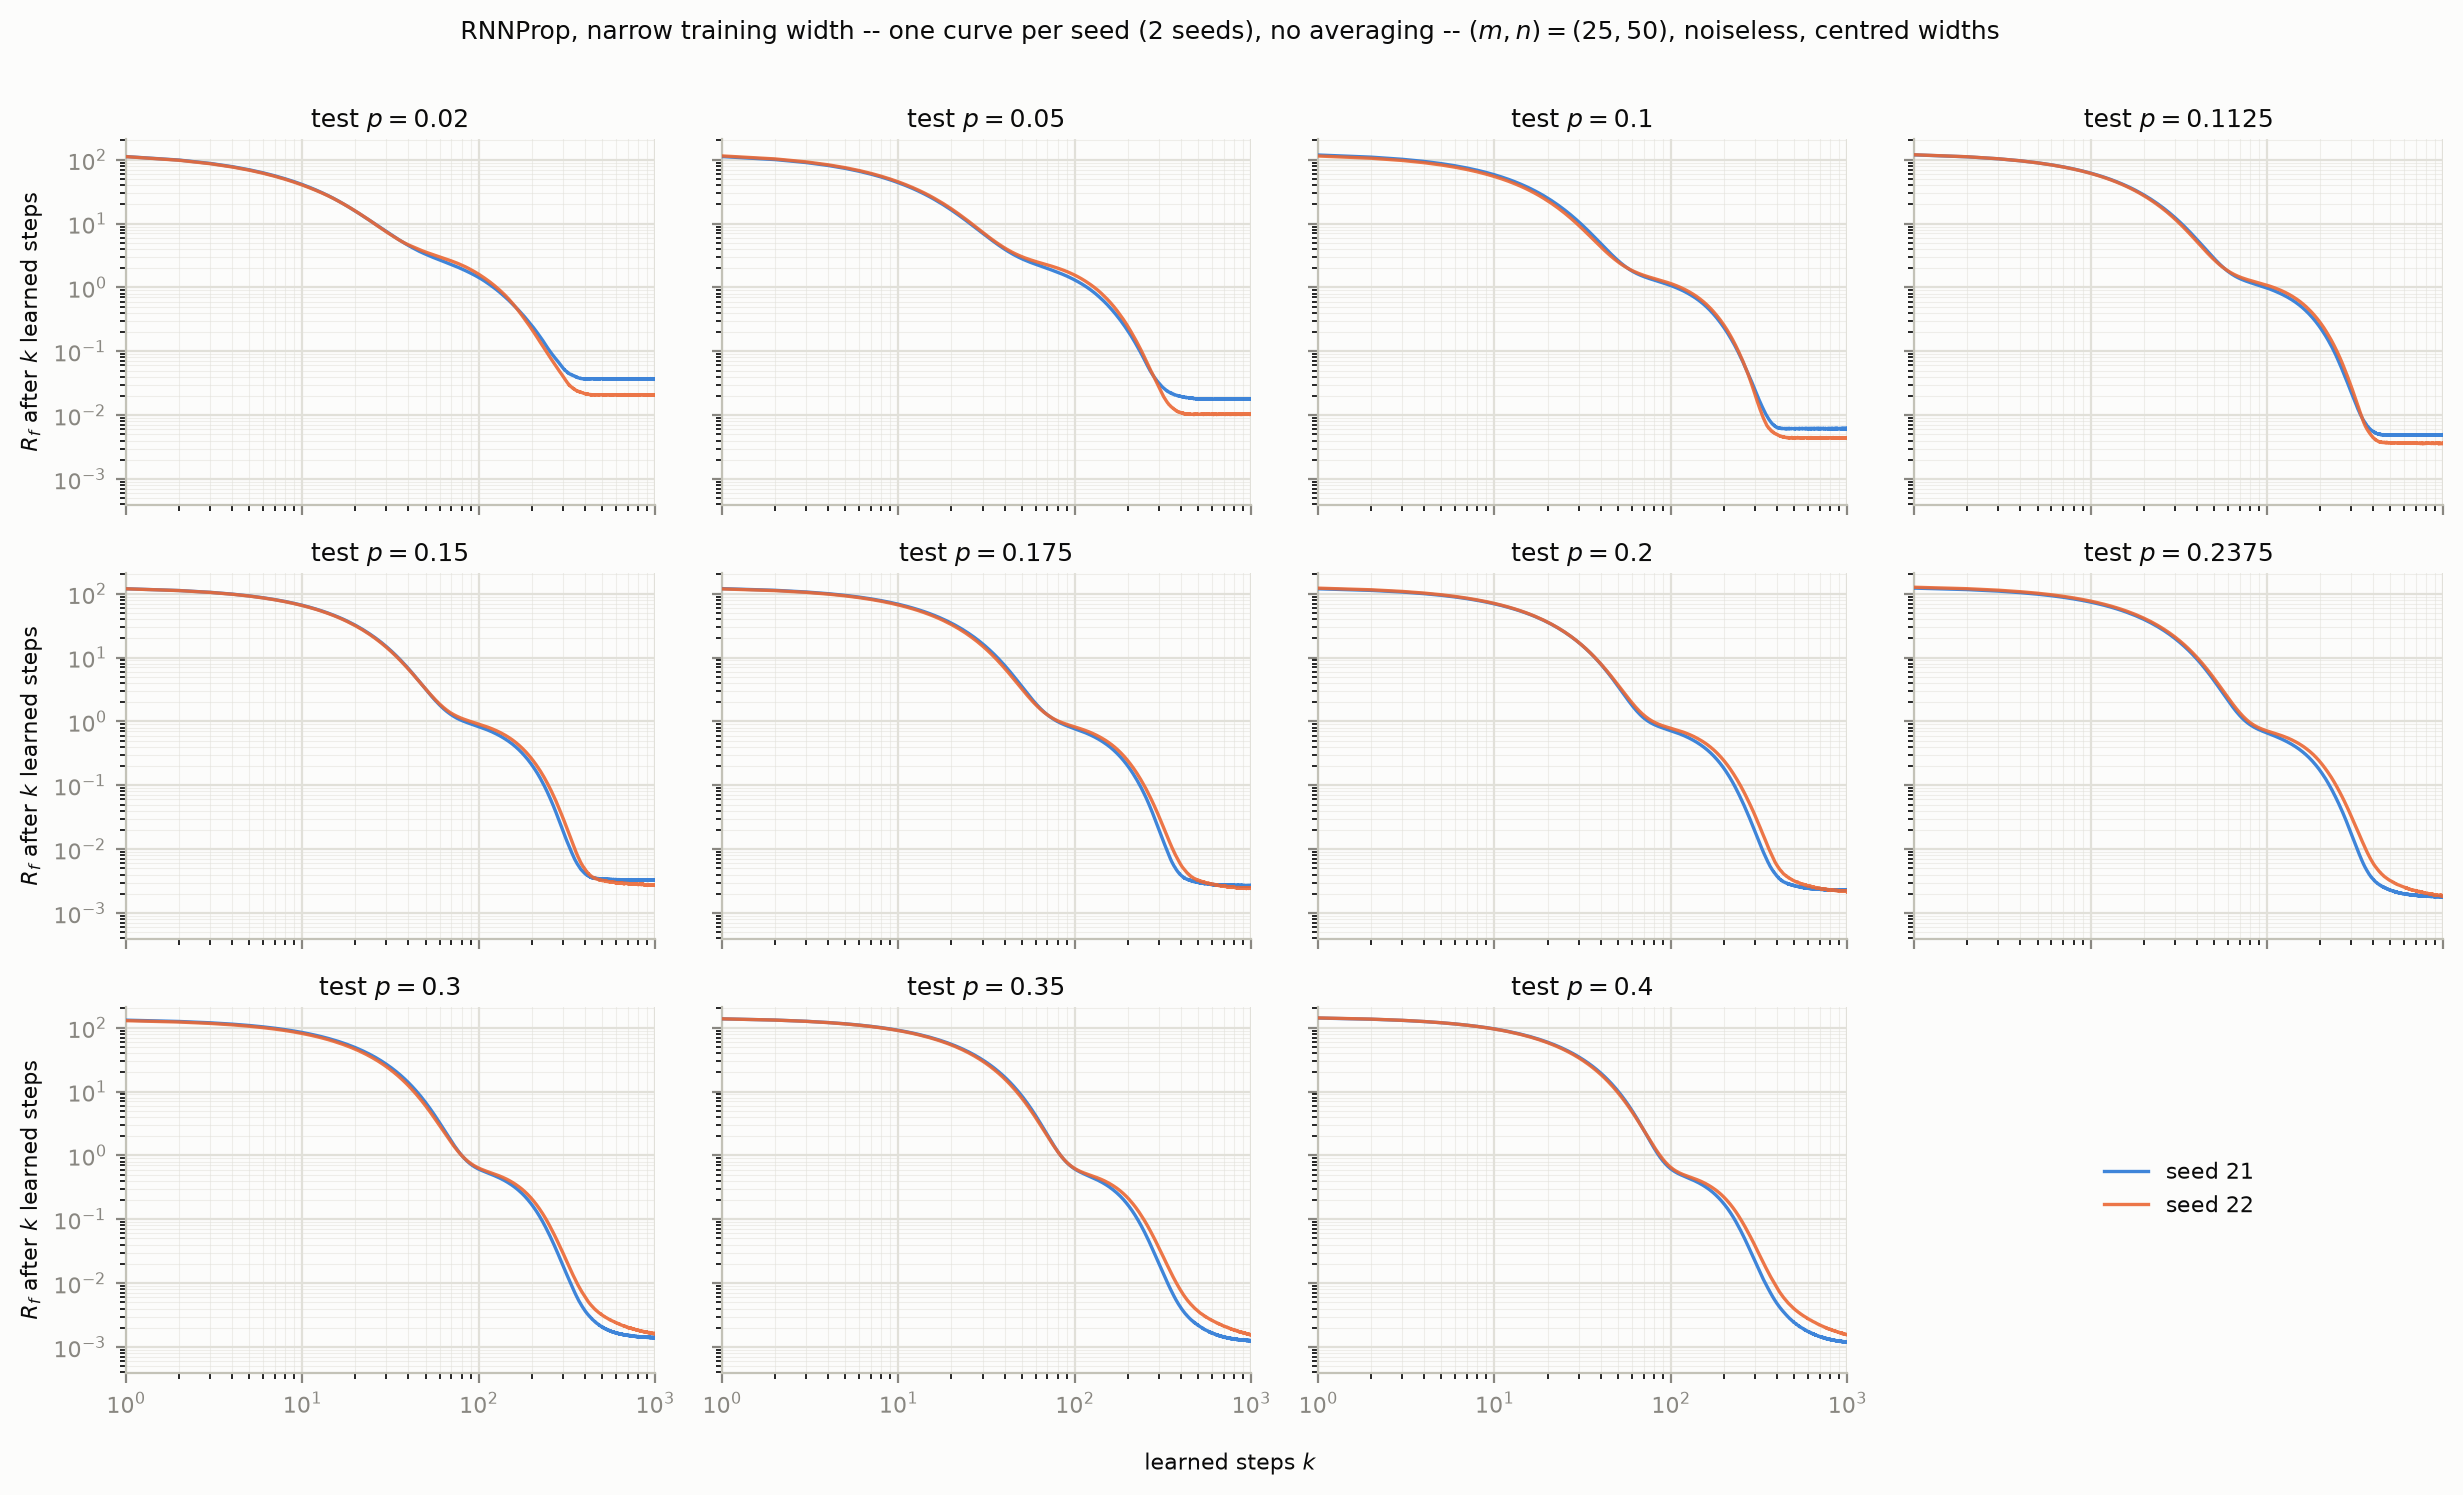
\includegraphics[width=\linewidth]{Figs/exp2_try2/rnnprop_seed_curves_exp2_try2_narrow.png}
  \caption{Narrow ($p = 0.175$)}
  \label{fig:rnnprop-seed-curves-exp2-try2-narrow}
\end{subfigure}\\[6pt]
\begin{subfigure}[t]{\linewidth}
  \centering
  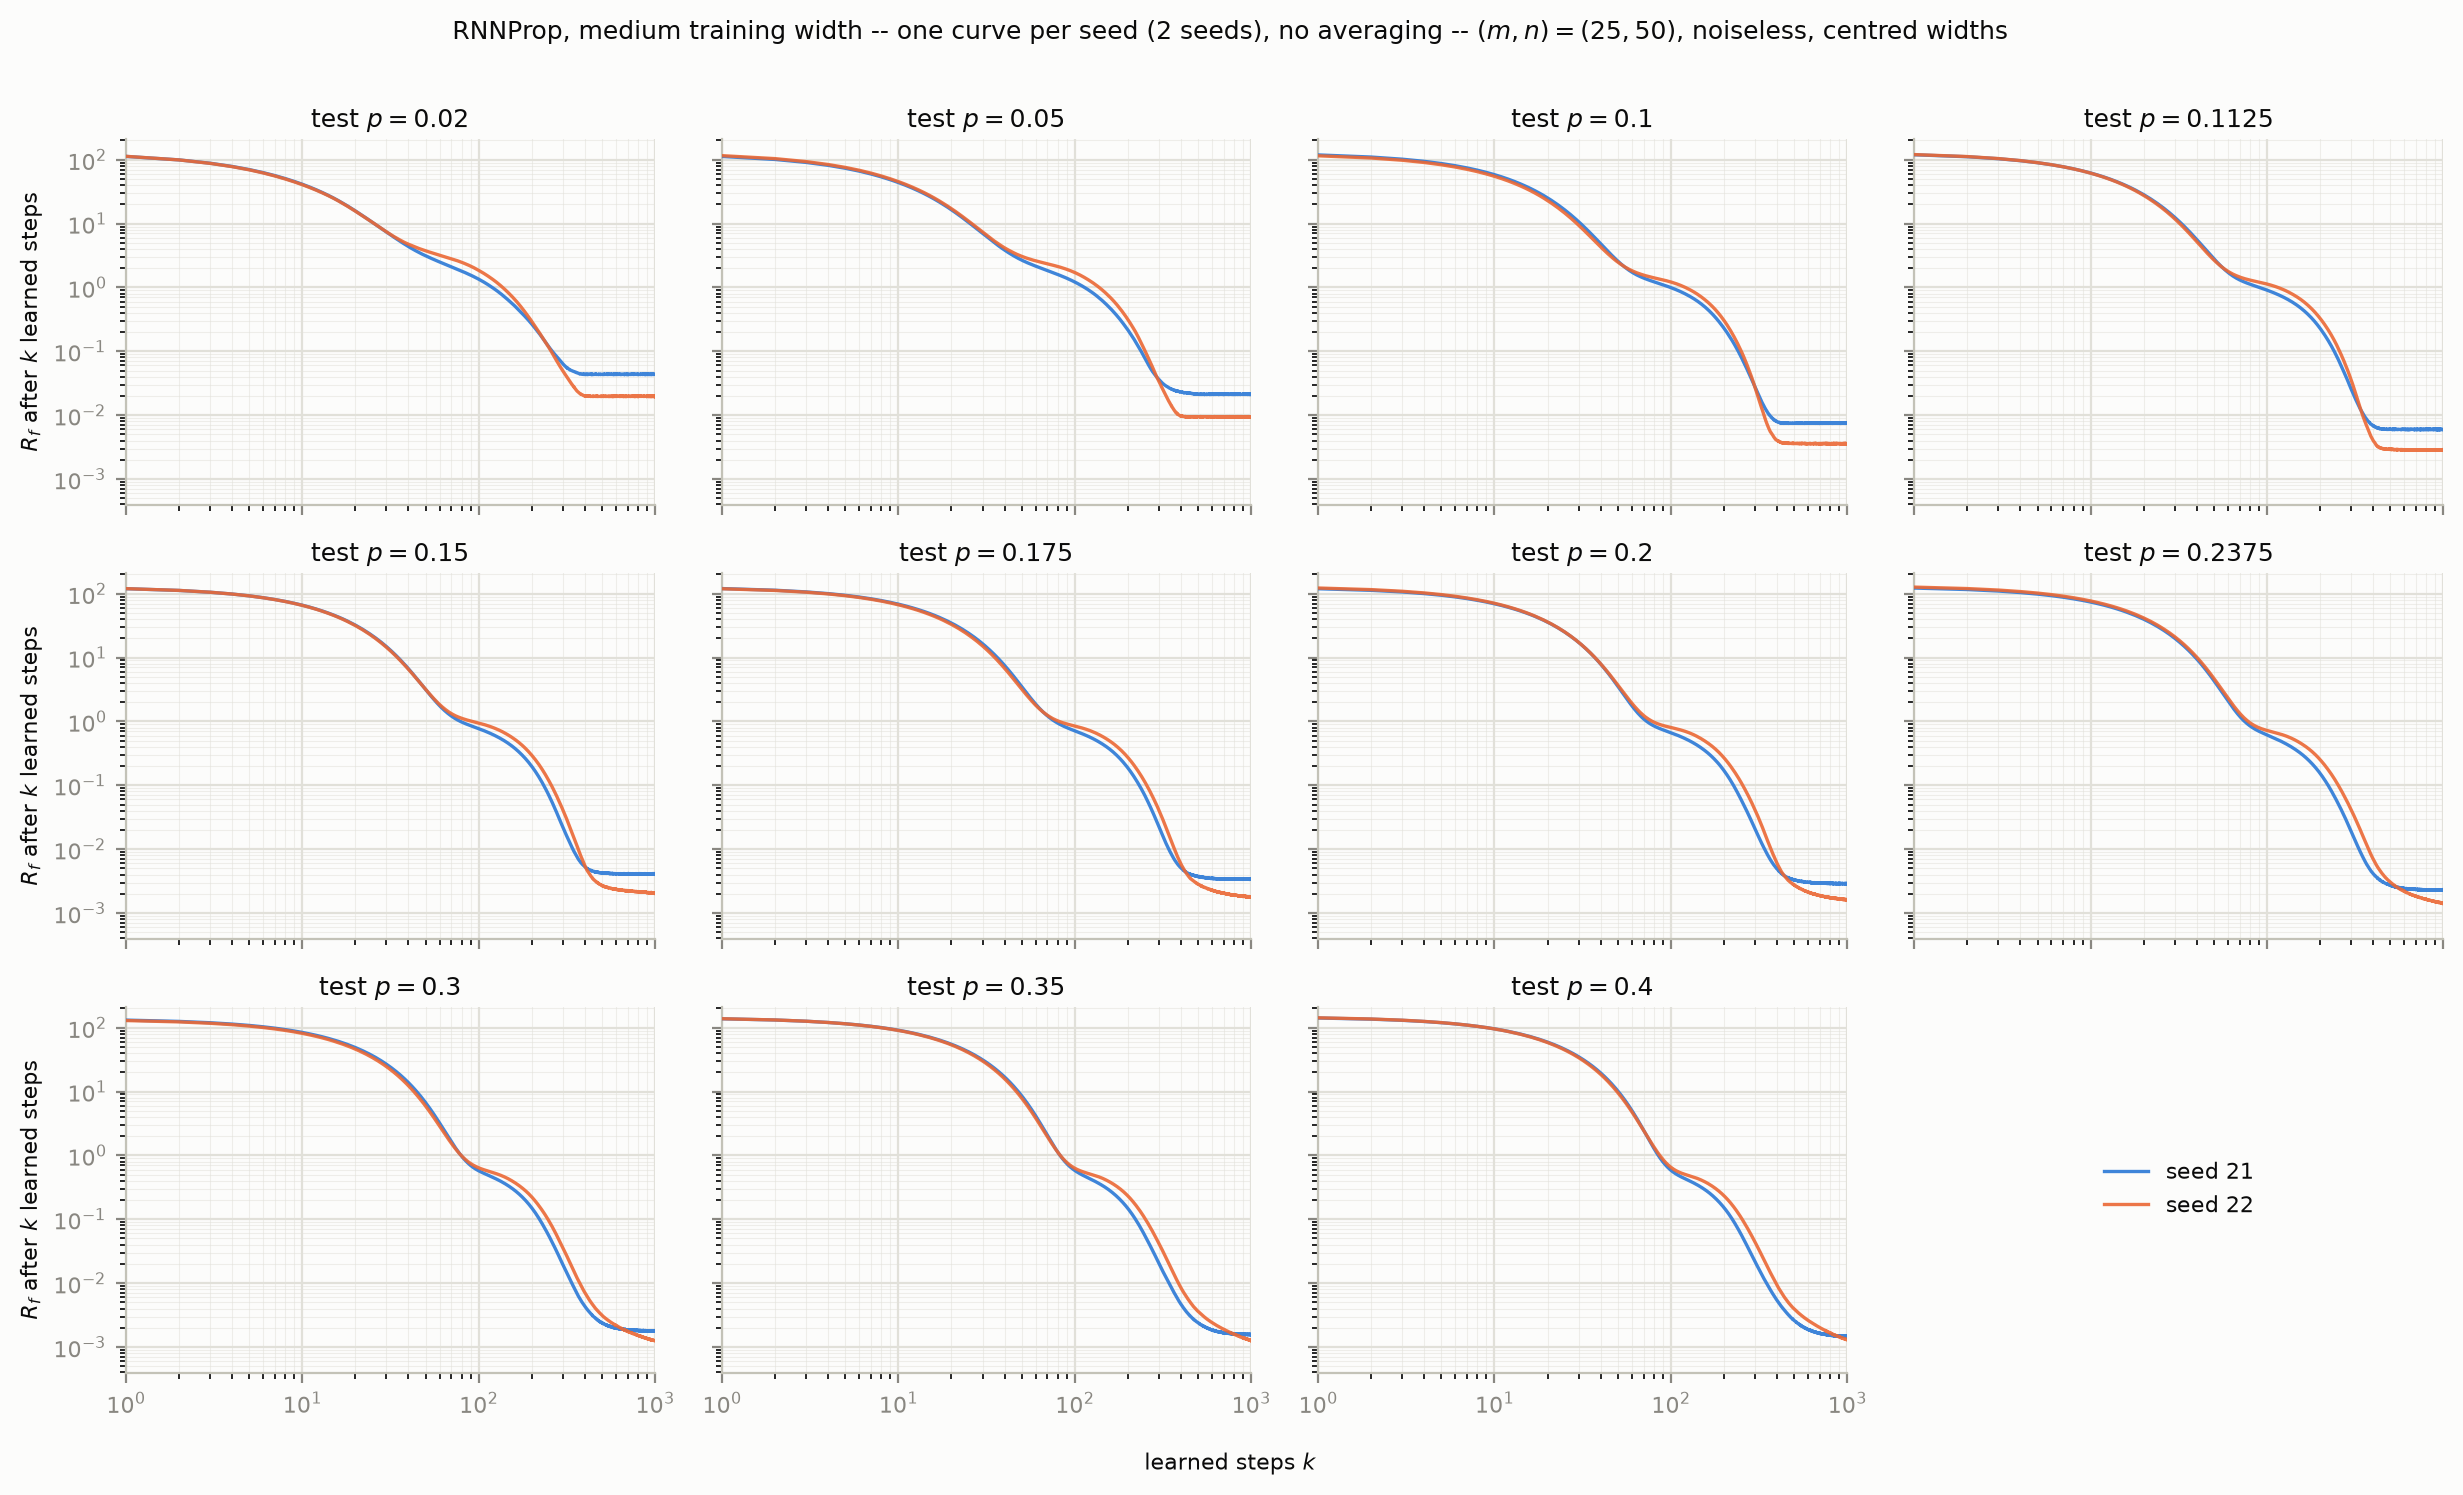
\includegraphics[width=\linewidth]{Figs/exp2_try2/rnnprop_seed_curves_exp2_try2_medium.png}
  \caption{Medium ($p \in [0.1125, 0.2375]$)}
  \label{fig:rnnprop-seed-curves-exp2-try2-medium}
\end{subfigure}\\[6pt]
\begin{subfigure}[t]{\linewidth}
  \centering
  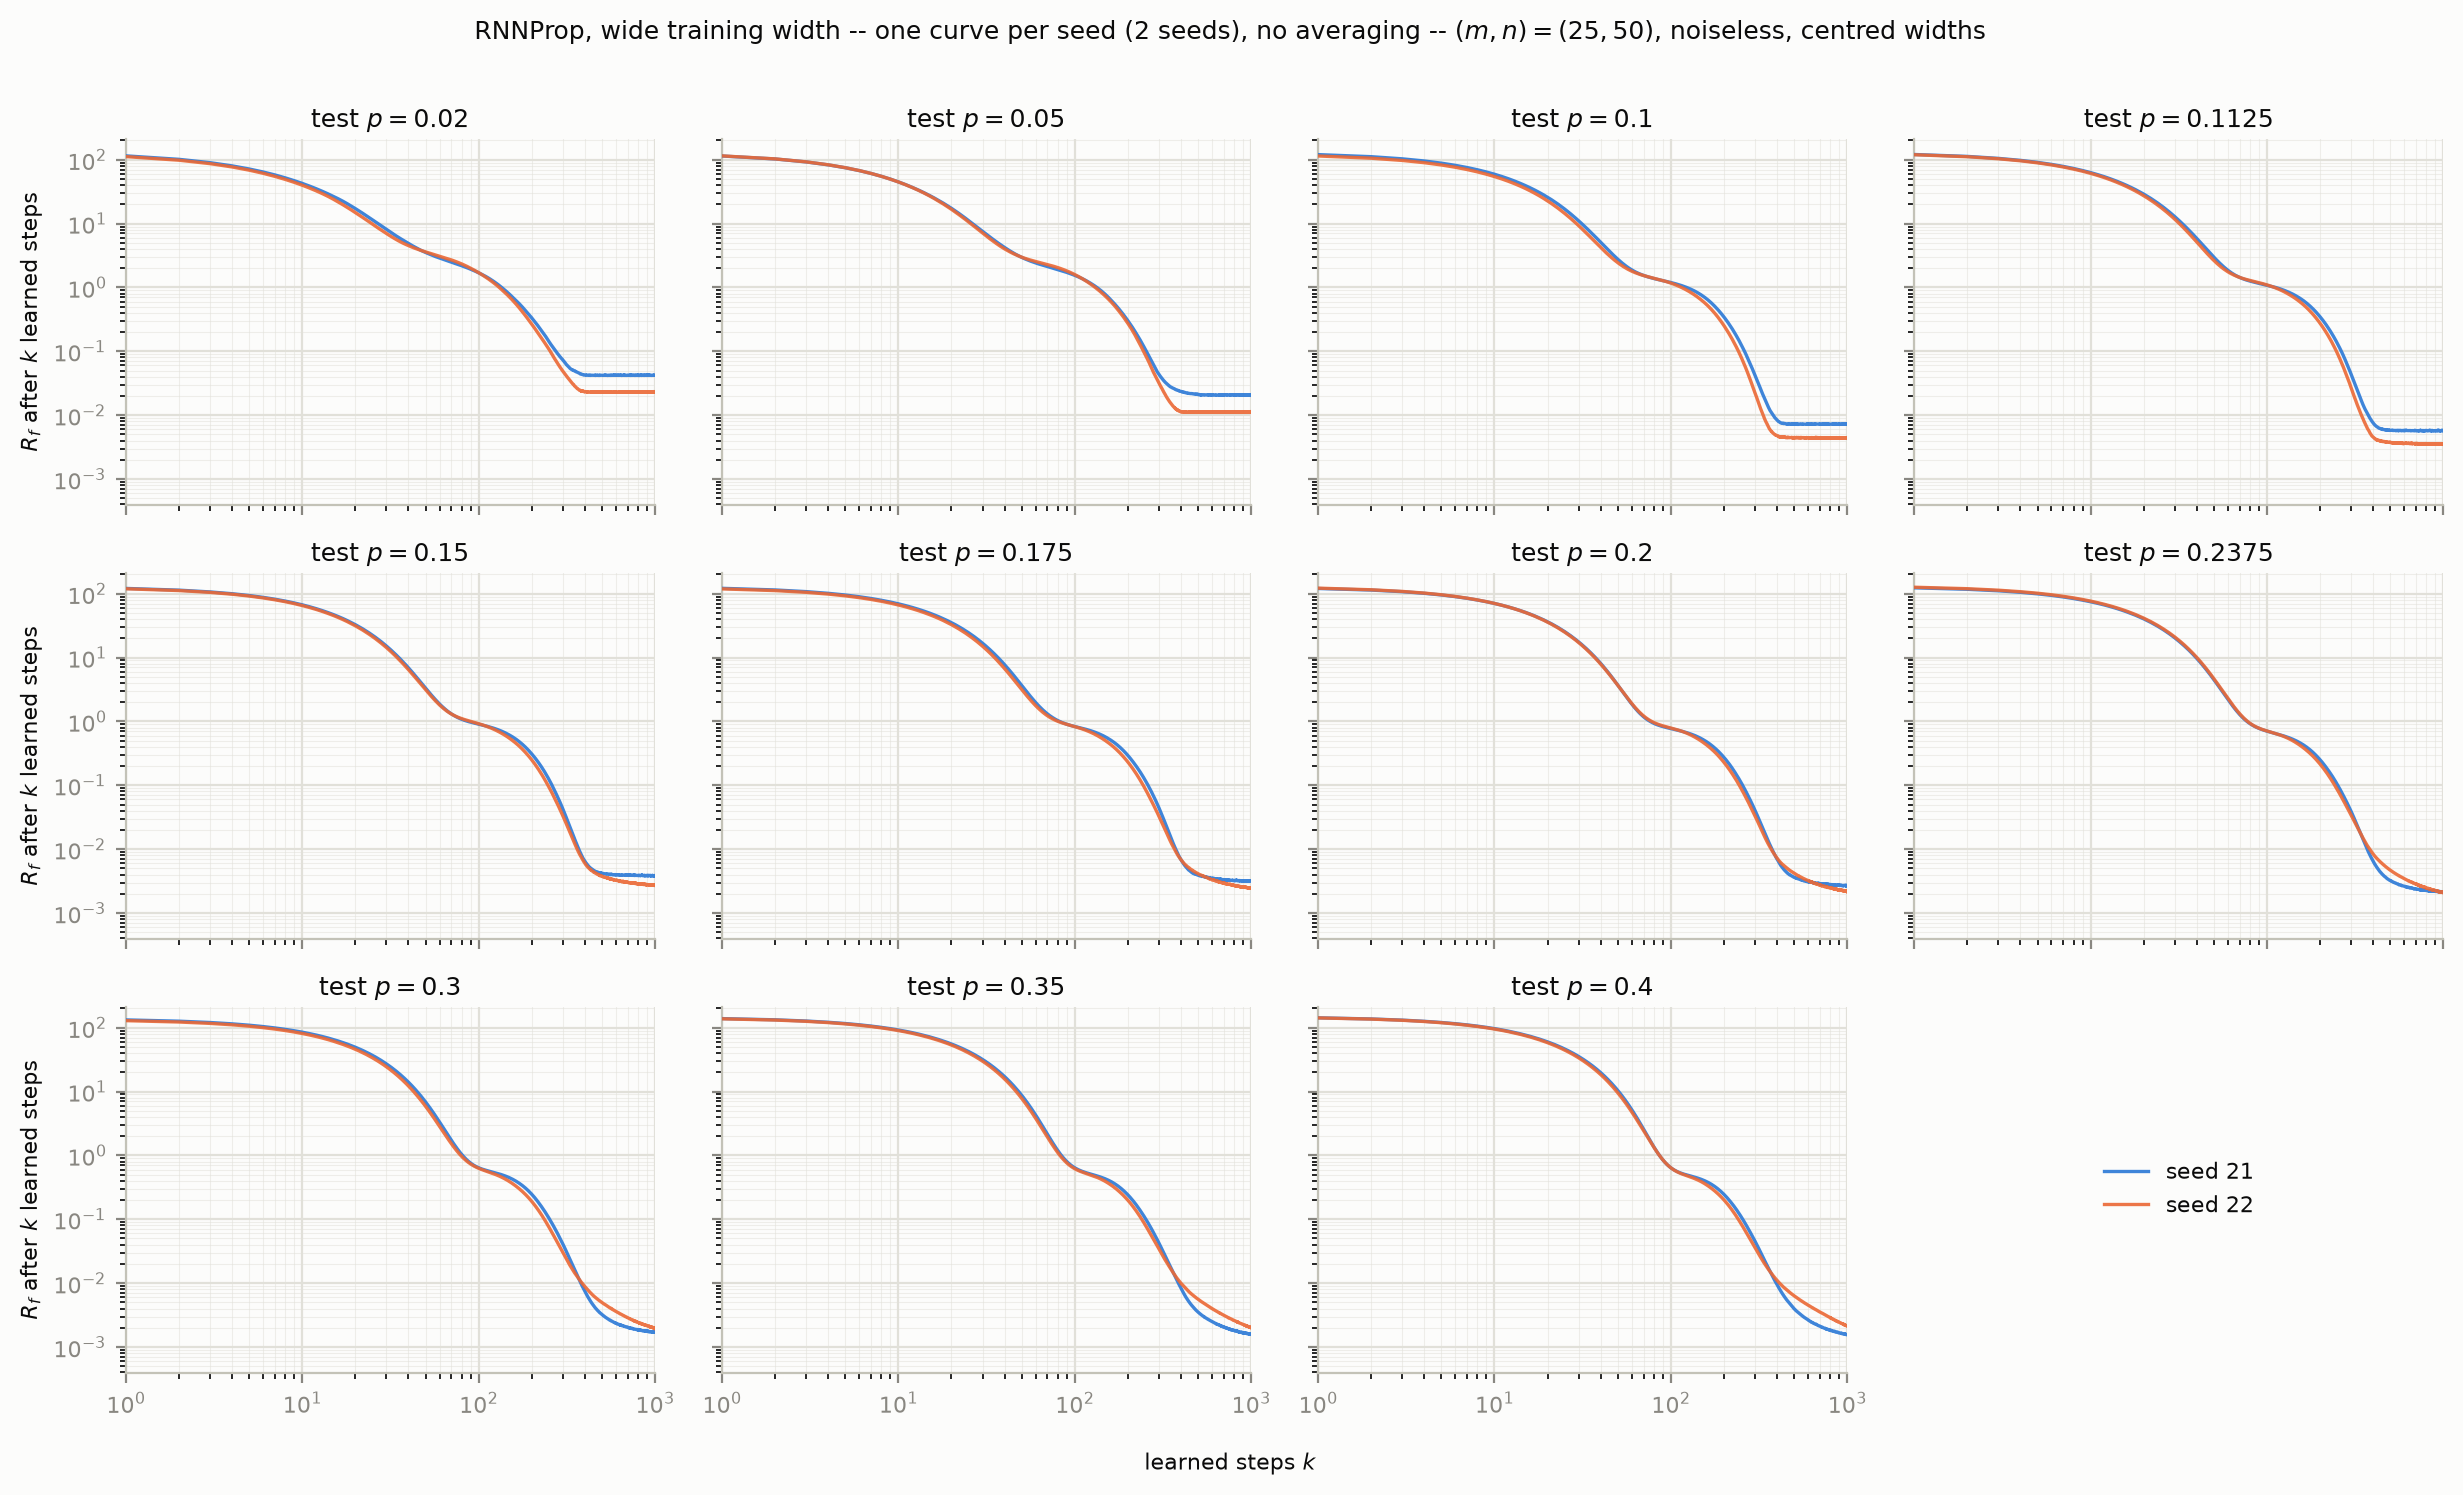
\includegraphics[width=\linewidth]{Figs/exp2_try2/rnnprop_seed_curves_exp2_try2_wide.png}
  \caption{Wide ($p \in [0.05, 0.30]$)}
  \label{fig:rnnprop-seed-curves-exp2-try2-wide}
\end{subfigure}\\[6pt]
\caption{L2O-RNNProp, modified relative loss $R_f$ (Eq.~10) against learned steps, $(m,n) = (25, 50)$, noiseless, centred widths. One curve per training seed (2 independently trained optimizers per width), no averaging; one panel per test sparsity $p$. The curves of different seeds agree closely for the first $\sim$100--200 steps and separate only on the plateau: the early trajectory is set by the architecture's normalised inputs and bounded ($\tanh \times 0.01$) output rather than by the learned weights.}
\label{fig:rnnprop-seed-curves-exp2-try2}
\end{figure}

\begin{figure}[htbp]
\centering
\begin{subfigure}[t]{\linewidth}
  \centering
  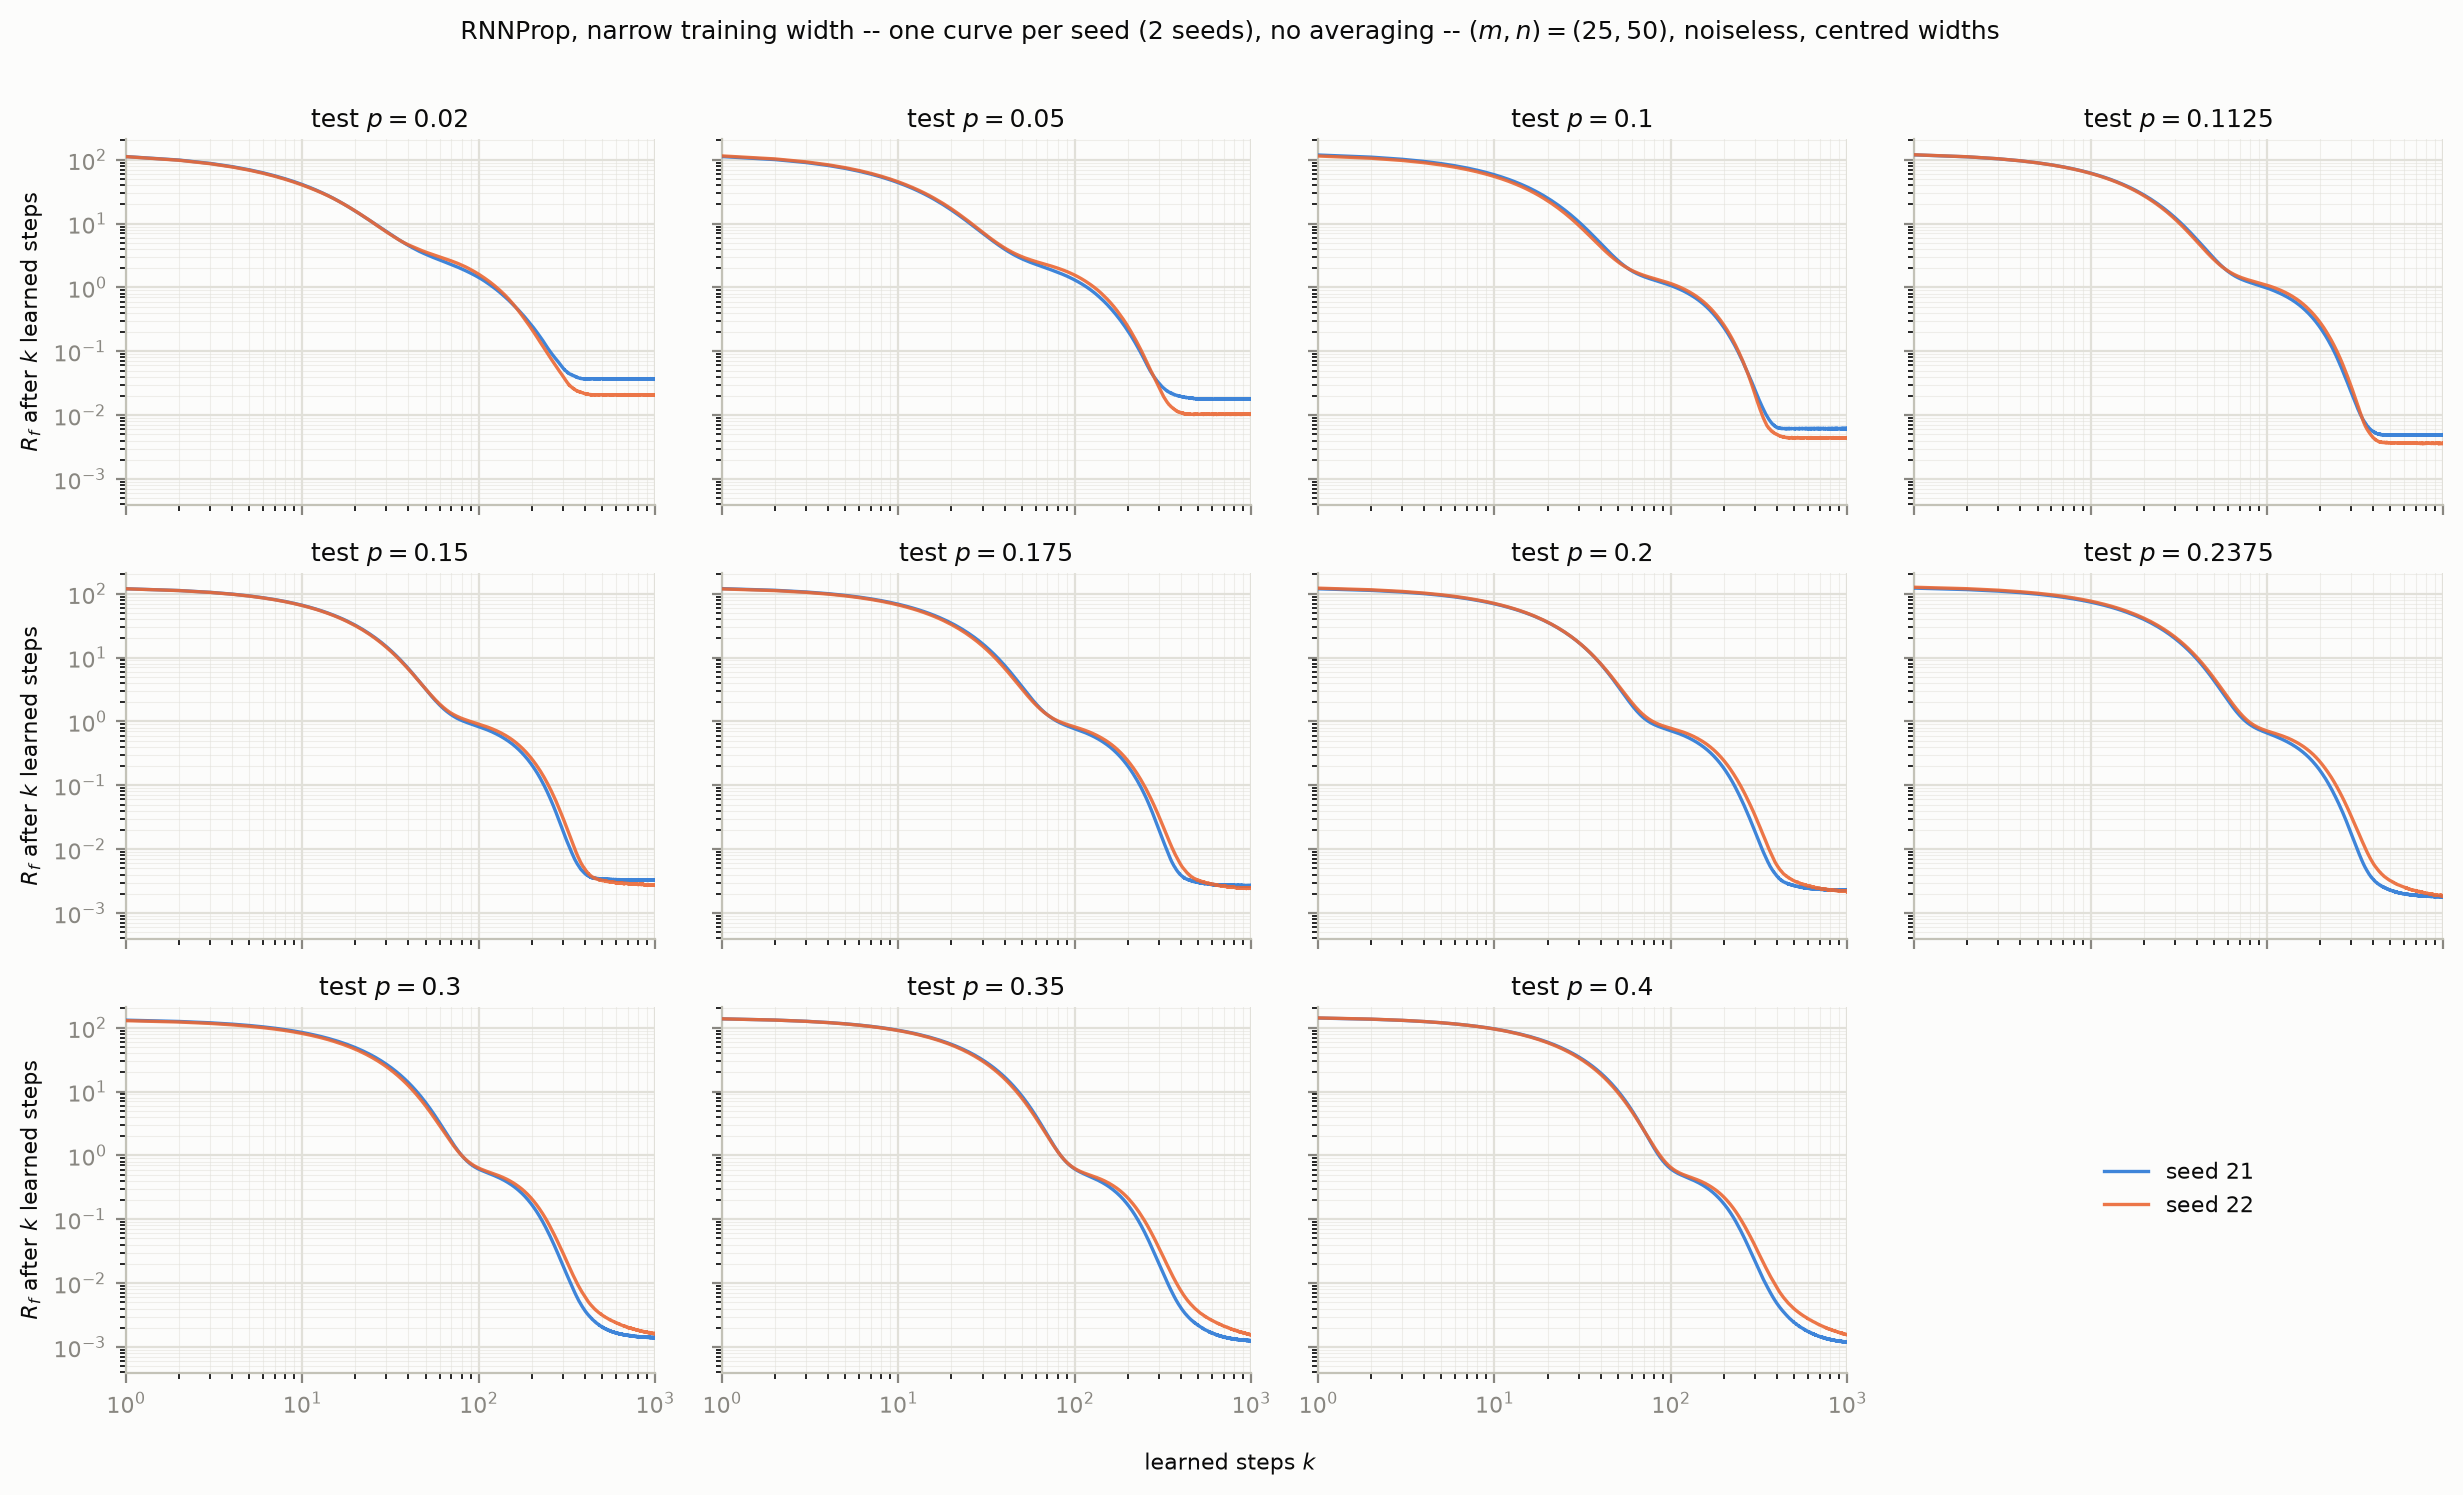
\includegraphics[width=\linewidth]{Figs/exp2_try2/rnnprop_seed_curves_exp2_try2_narrow.png}
  \caption{Narrow ($p = 0.175$)}
  \label{fig:rnnprop-seed-curves-exp2-try2-narrow}
\end{subfigure}\\[6pt]
\begin{subfigure}[t]{\linewidth}
  \centering
  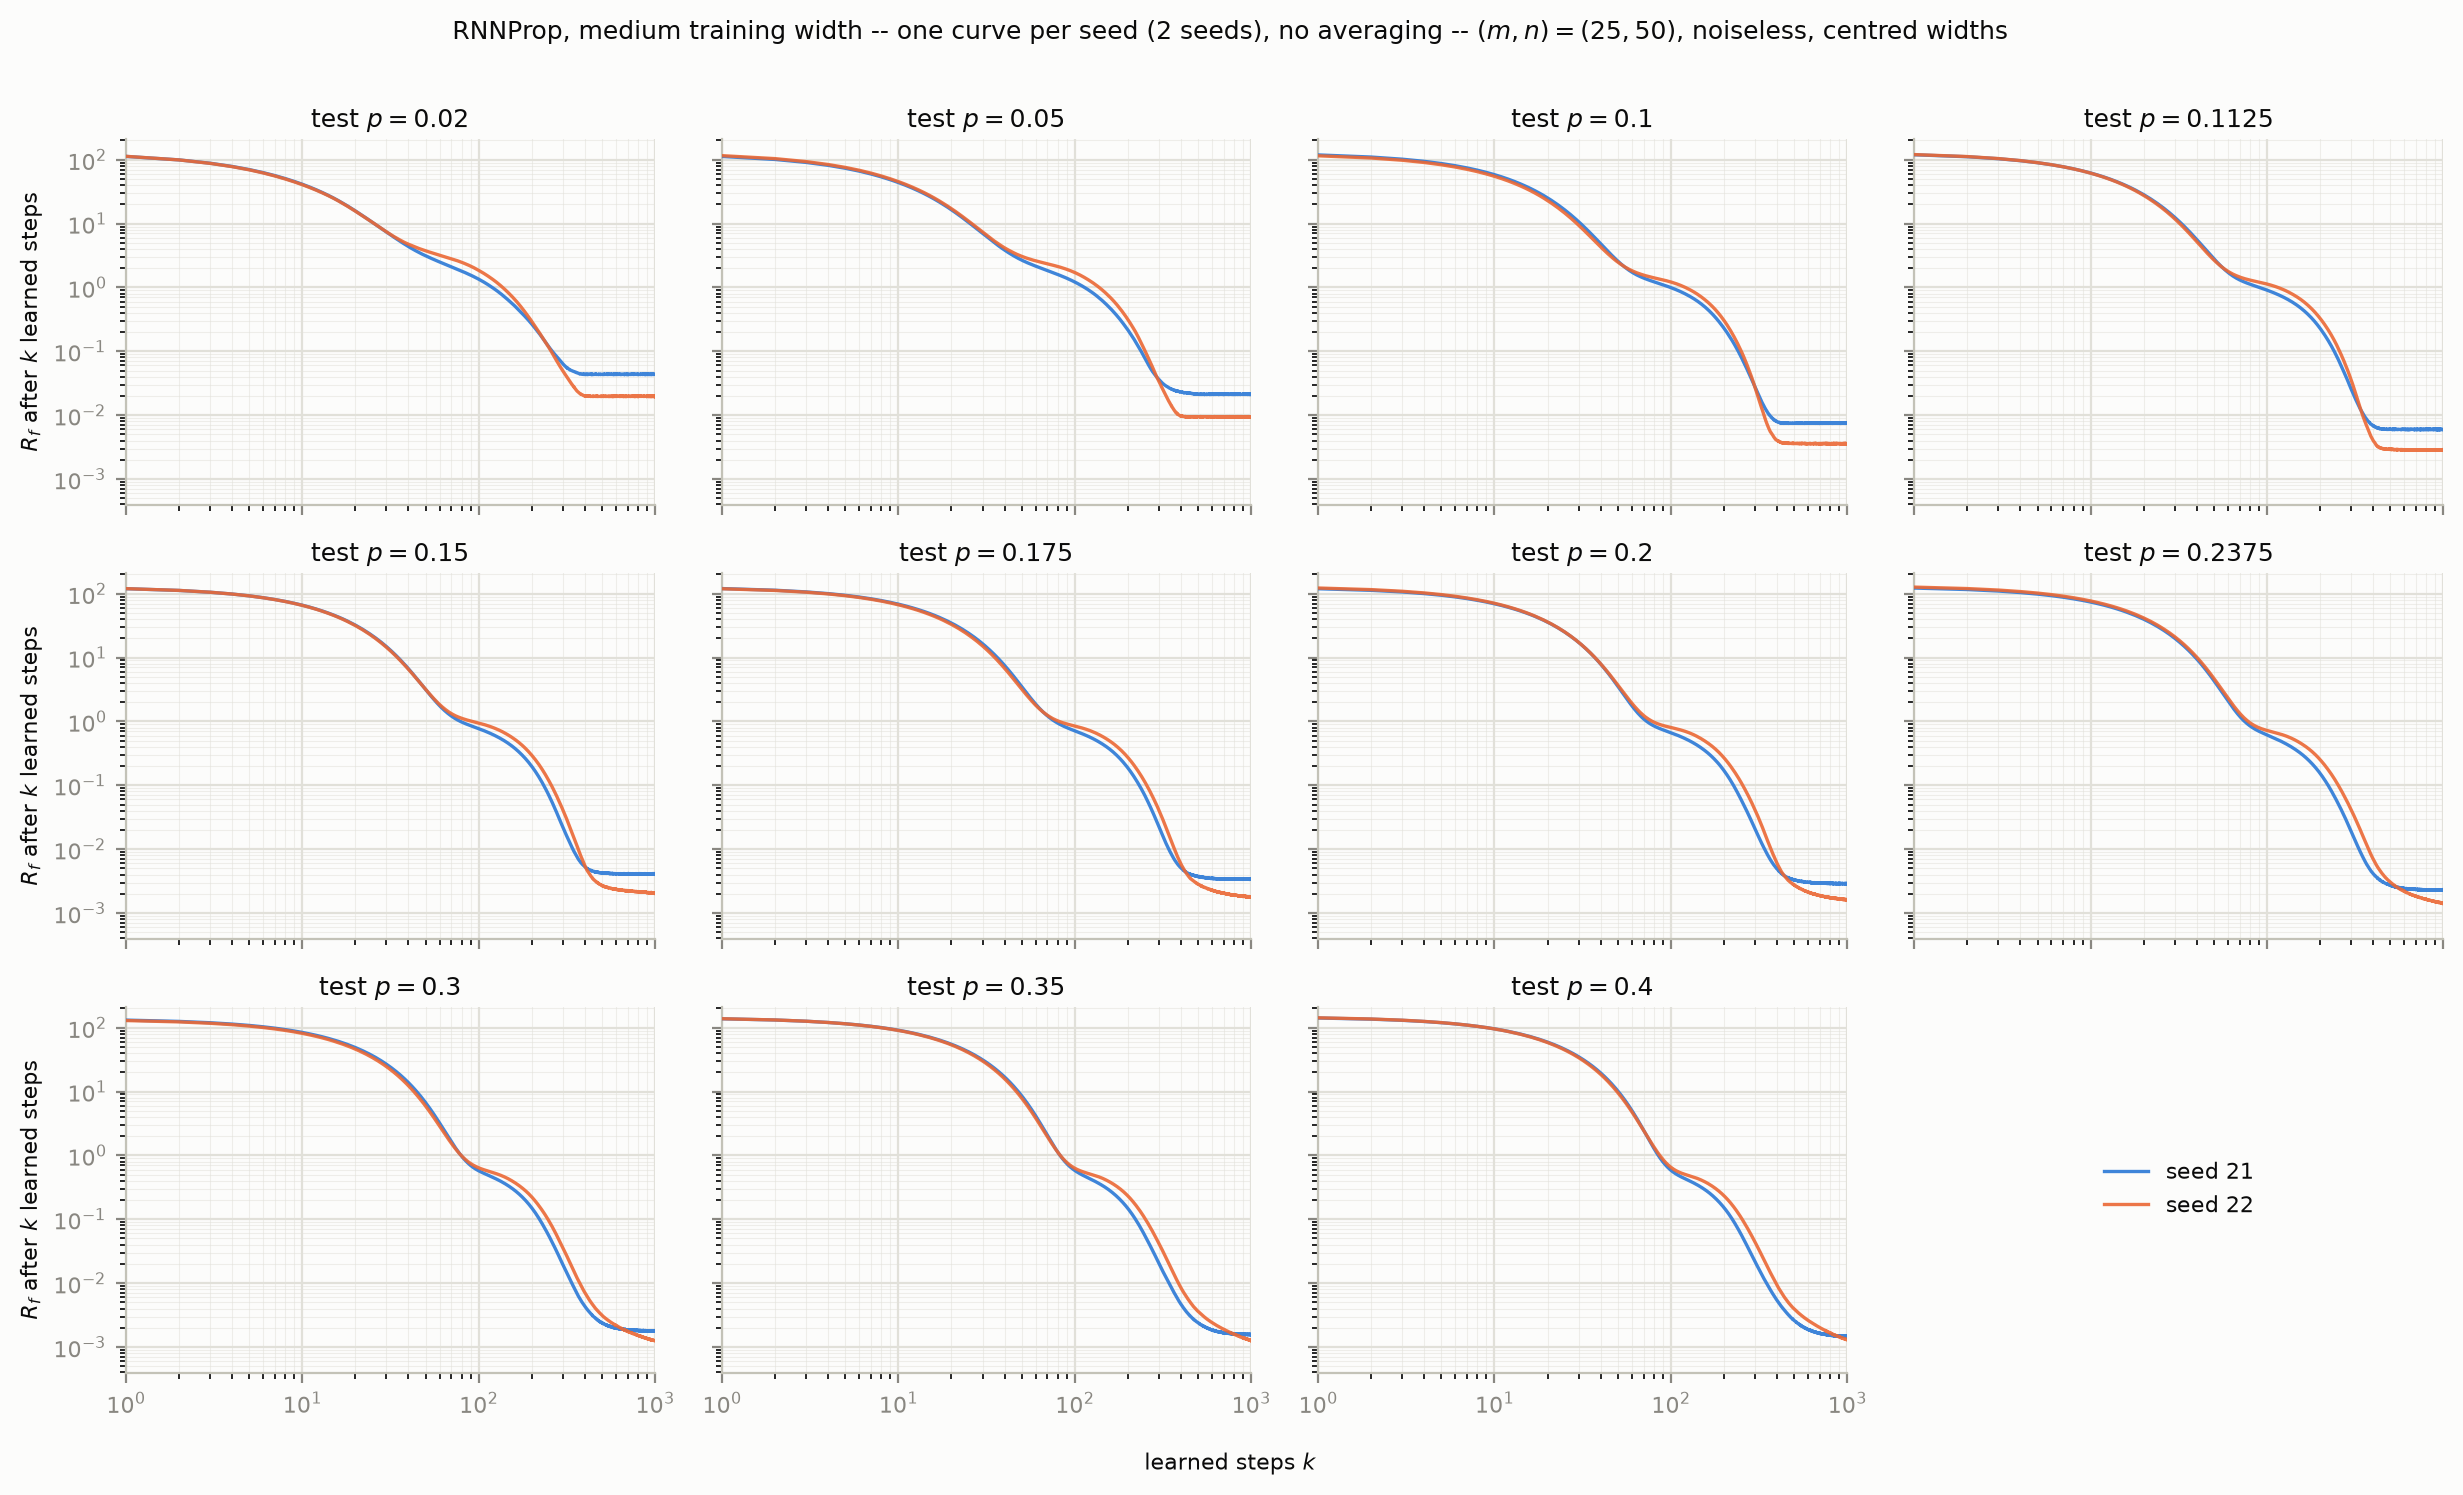
\includegraphics[width=\linewidth]{Figs/exp2_try2/rnnprop_seed_curves_exp2_try2_medium.png}
  \caption{Medium ($p \in [0.1125, 0.2375]$)}
  \label{fig:rnnprop-seed-curves-exp2-try2-medium}
\end{subfigure}\\[6pt]
\begin{subfigure}[t]{\linewidth}
  \centering
  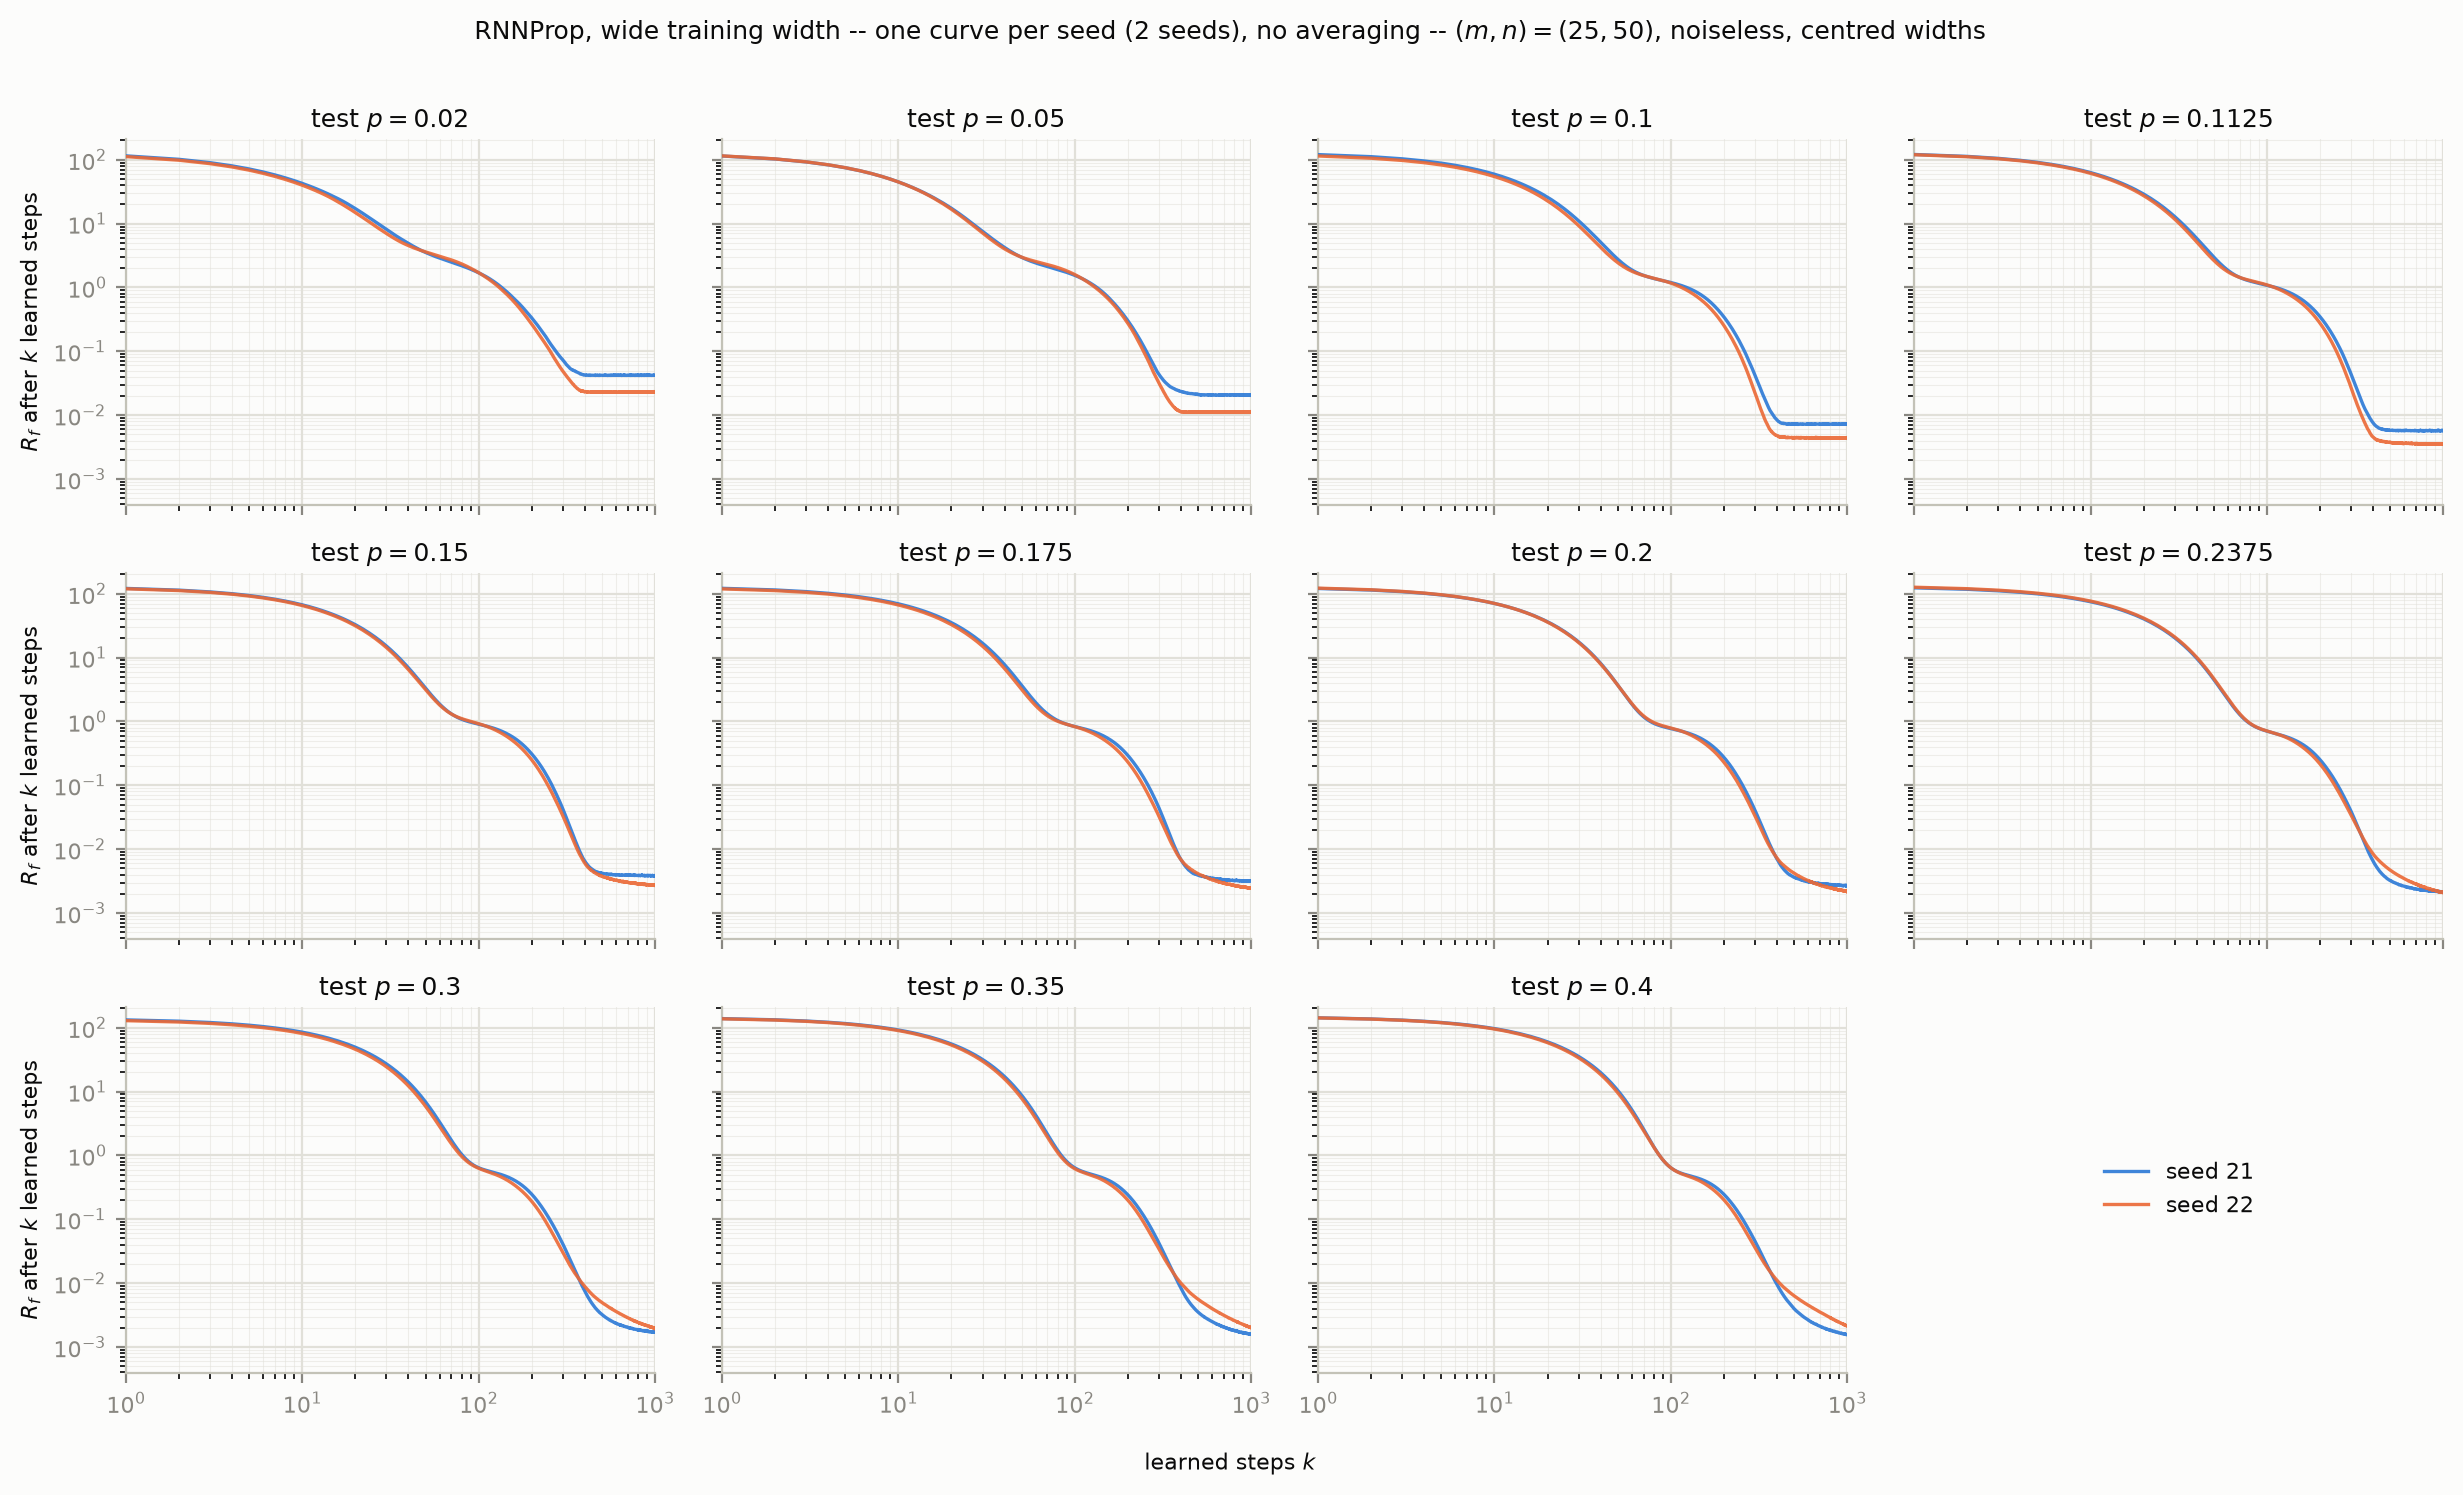
\includegraphics[width=\linewidth]{Figs/exp2_try2/rnnprop_seed_curves_exp2_try2_wide.png}
  \caption{Wide ($p \in [0.05, 0.30]$)}
  \label{fig:rnnprop-seed-curves-exp2-try2-wide}
\end{subfigure}\\[6pt]
\caption{L2O-RNNProp, modified relative loss $R_f$ (Eq.~10) against learned steps, $(m,n) = (25, 50)$, noiseless, centred widths. One curve per training seed (2 independently trained optimizers per width), no averaging; one panel per test sparsity $p$. The curves of different seeds agree closely for the first $\sim$100--200 steps and separate only on the plateau: the early trajectory is set by the architecture's normalised inputs and bounded ($\tanh \times 0.01$) output rather than by the learned weights.}
\label{fig:rnnprop-seed-curves-exp2-try2}
\end{figure}

\begin{figure}[htbp]
\centering
\begin{subfigure}[t]{\linewidth}
  \centering
  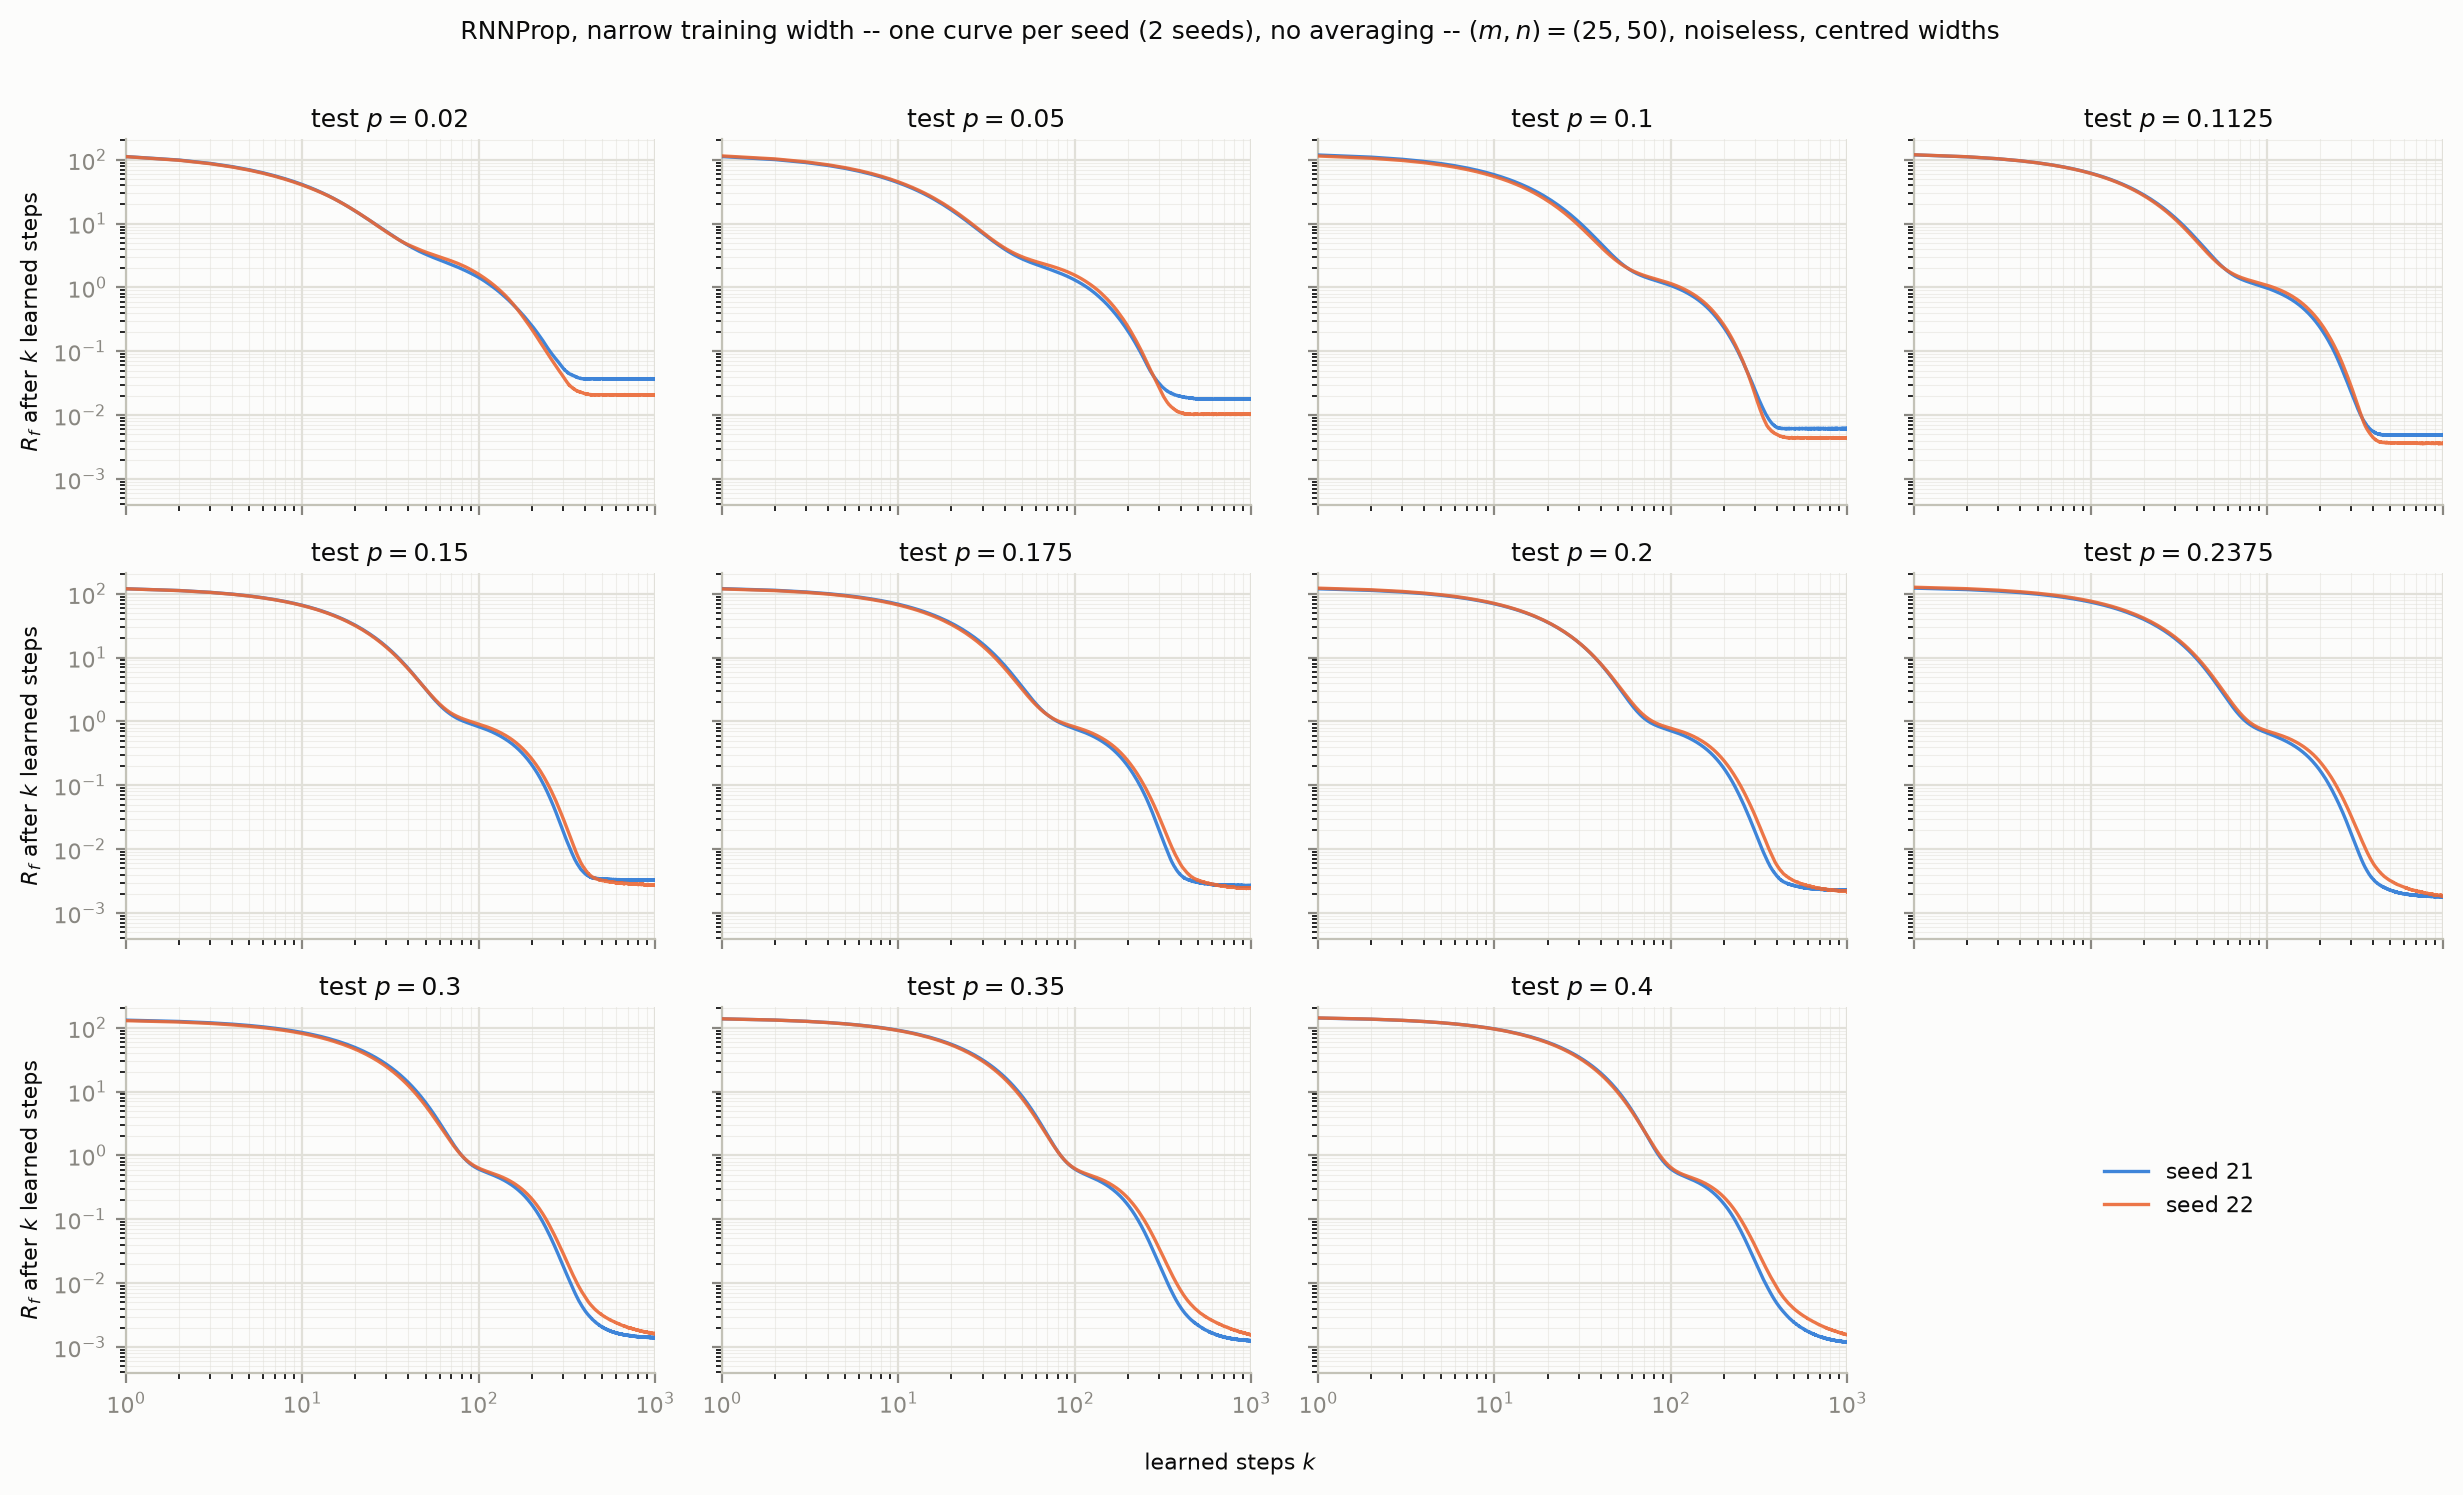
\includegraphics[width=\linewidth]{Figs/exp2_try2/rnnprop_seed_curves_exp2_try2_narrow.png}
  \caption{Narrow ($p = 0.175$)}
  \label{fig:rnnprop-seed-curves-exp2-try2-narrow}
\end{subfigure}\\[6pt]
\begin{subfigure}[t]{\linewidth}
  \centering
  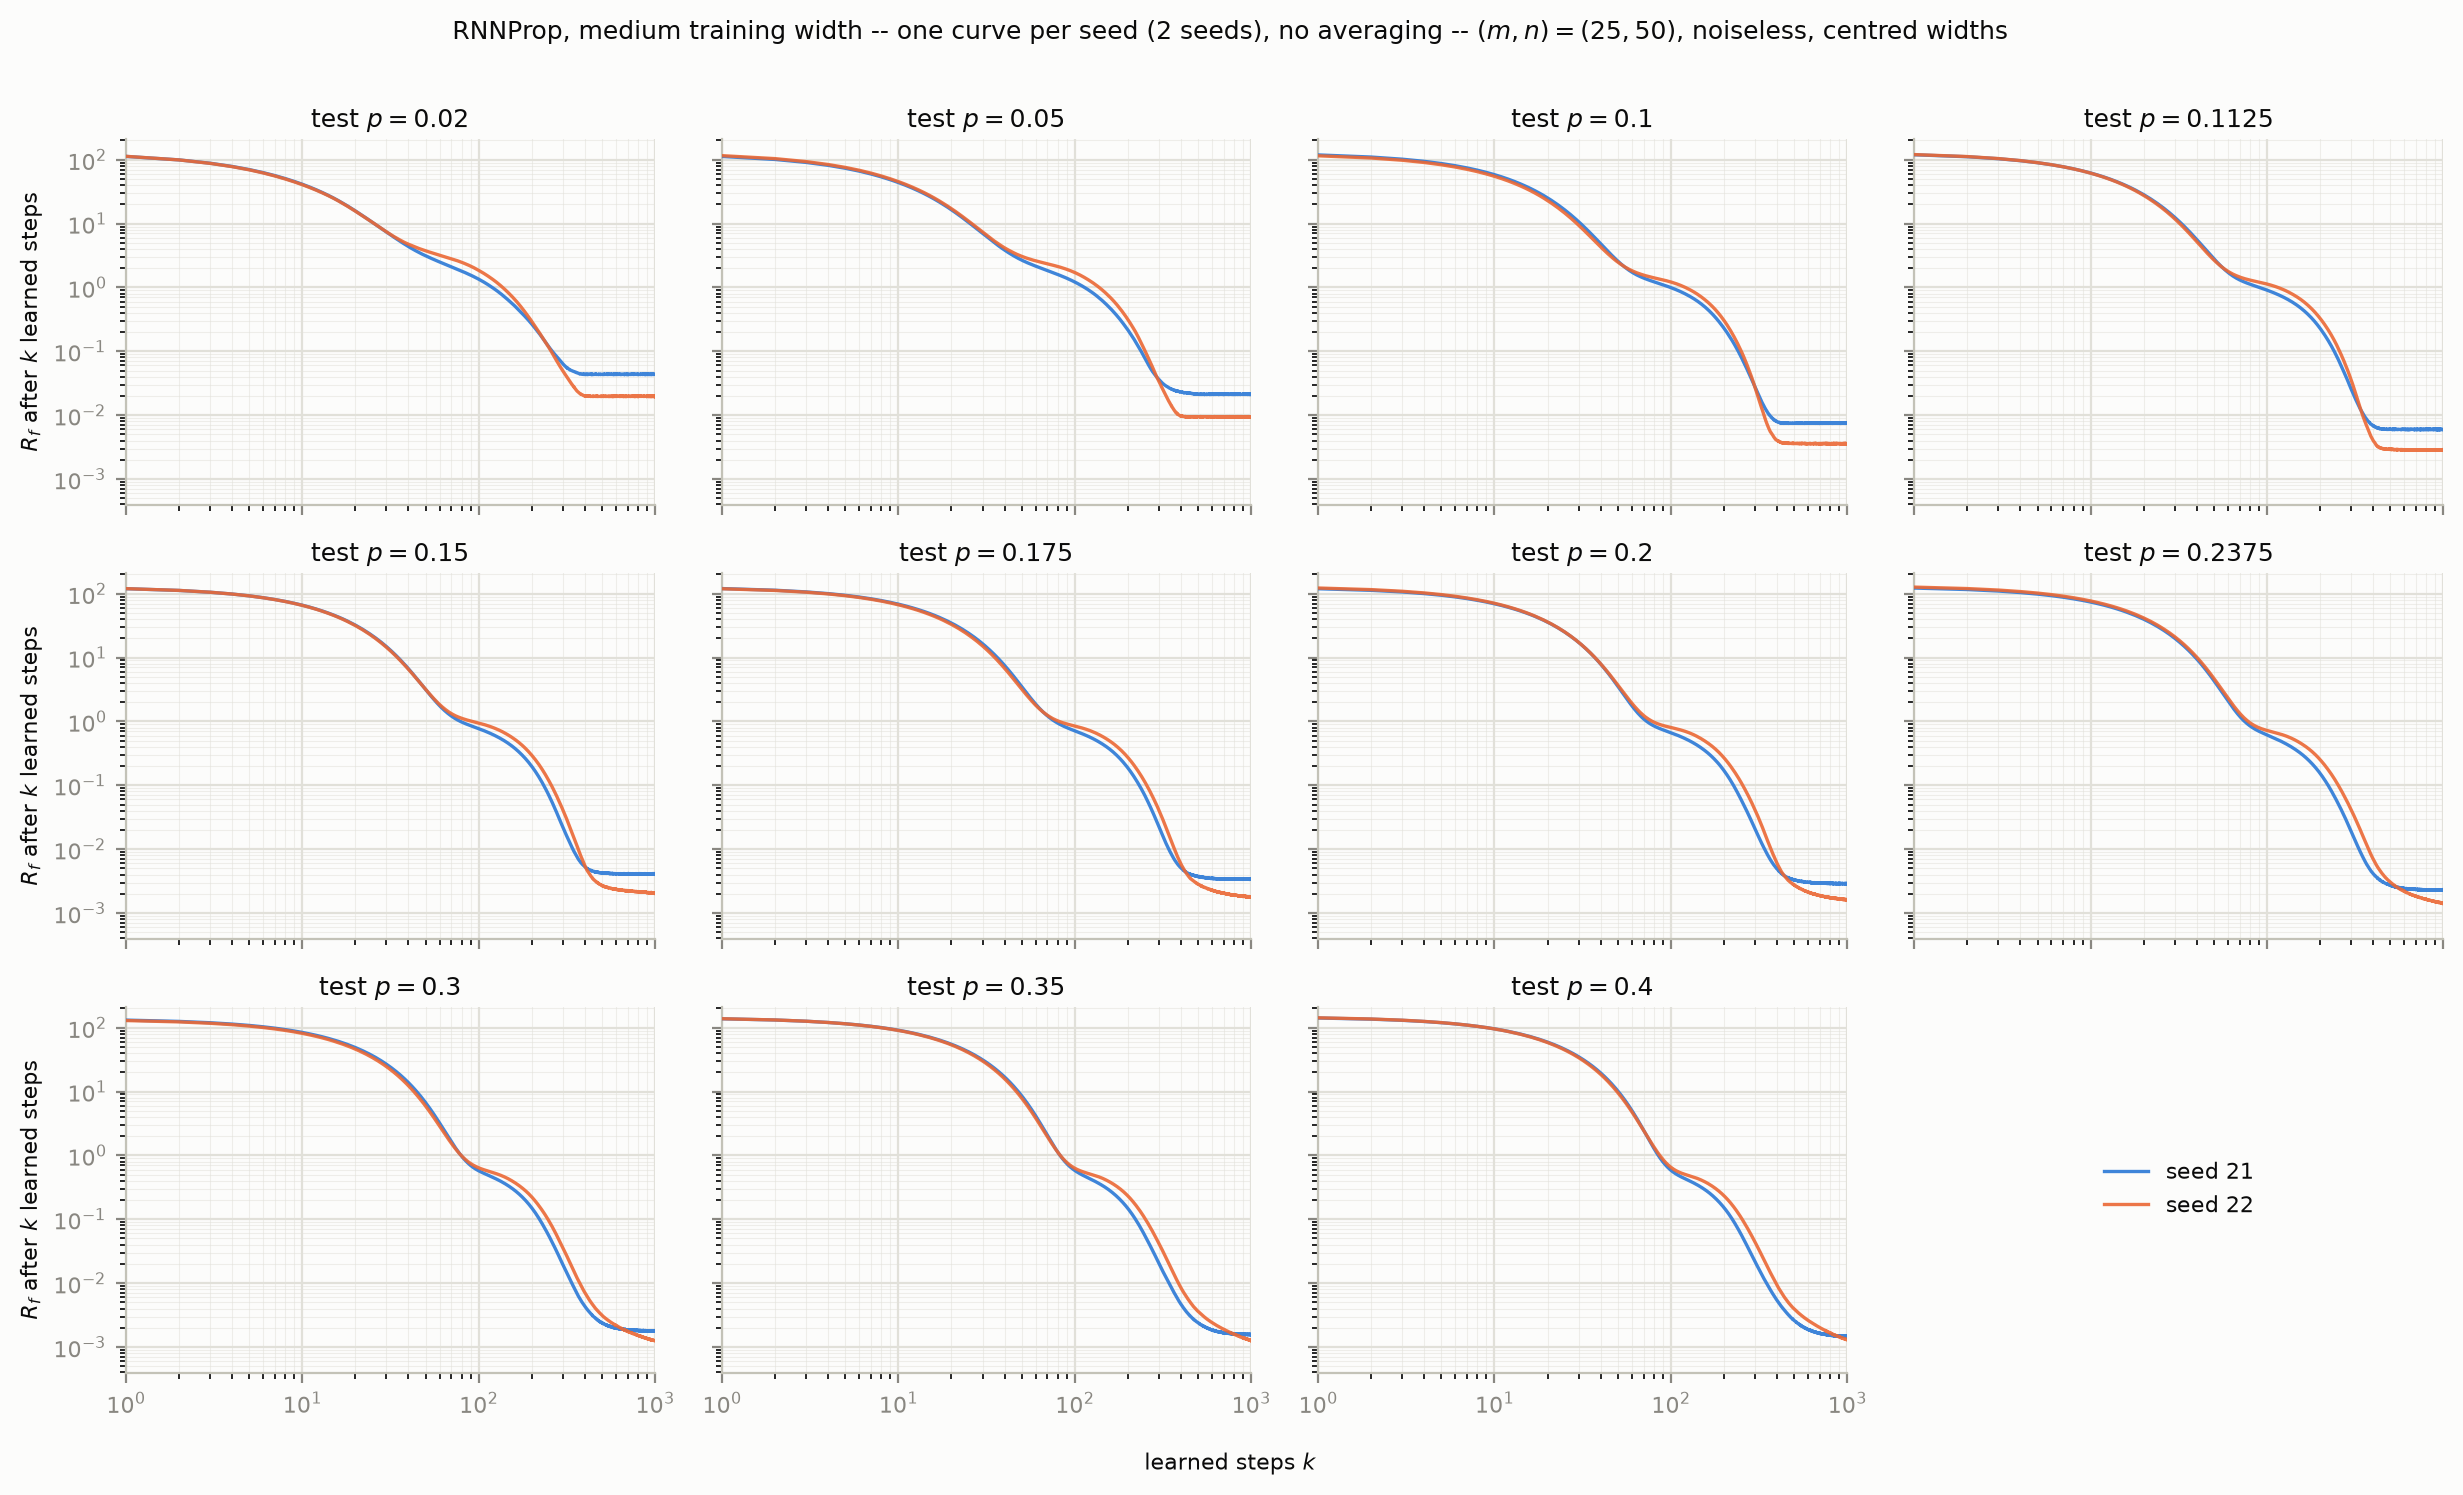
\includegraphics[width=\linewidth]{Figs/exp2_try2/rnnprop_seed_curves_exp2_try2_medium.png}
  \caption{Medium ($p \in [0.1125, 0.2375]$)}
  \label{fig:rnnprop-seed-curves-exp2-try2-medium}
\end{subfigure}\\[6pt]
\begin{subfigure}[t]{\linewidth}
  \centering
  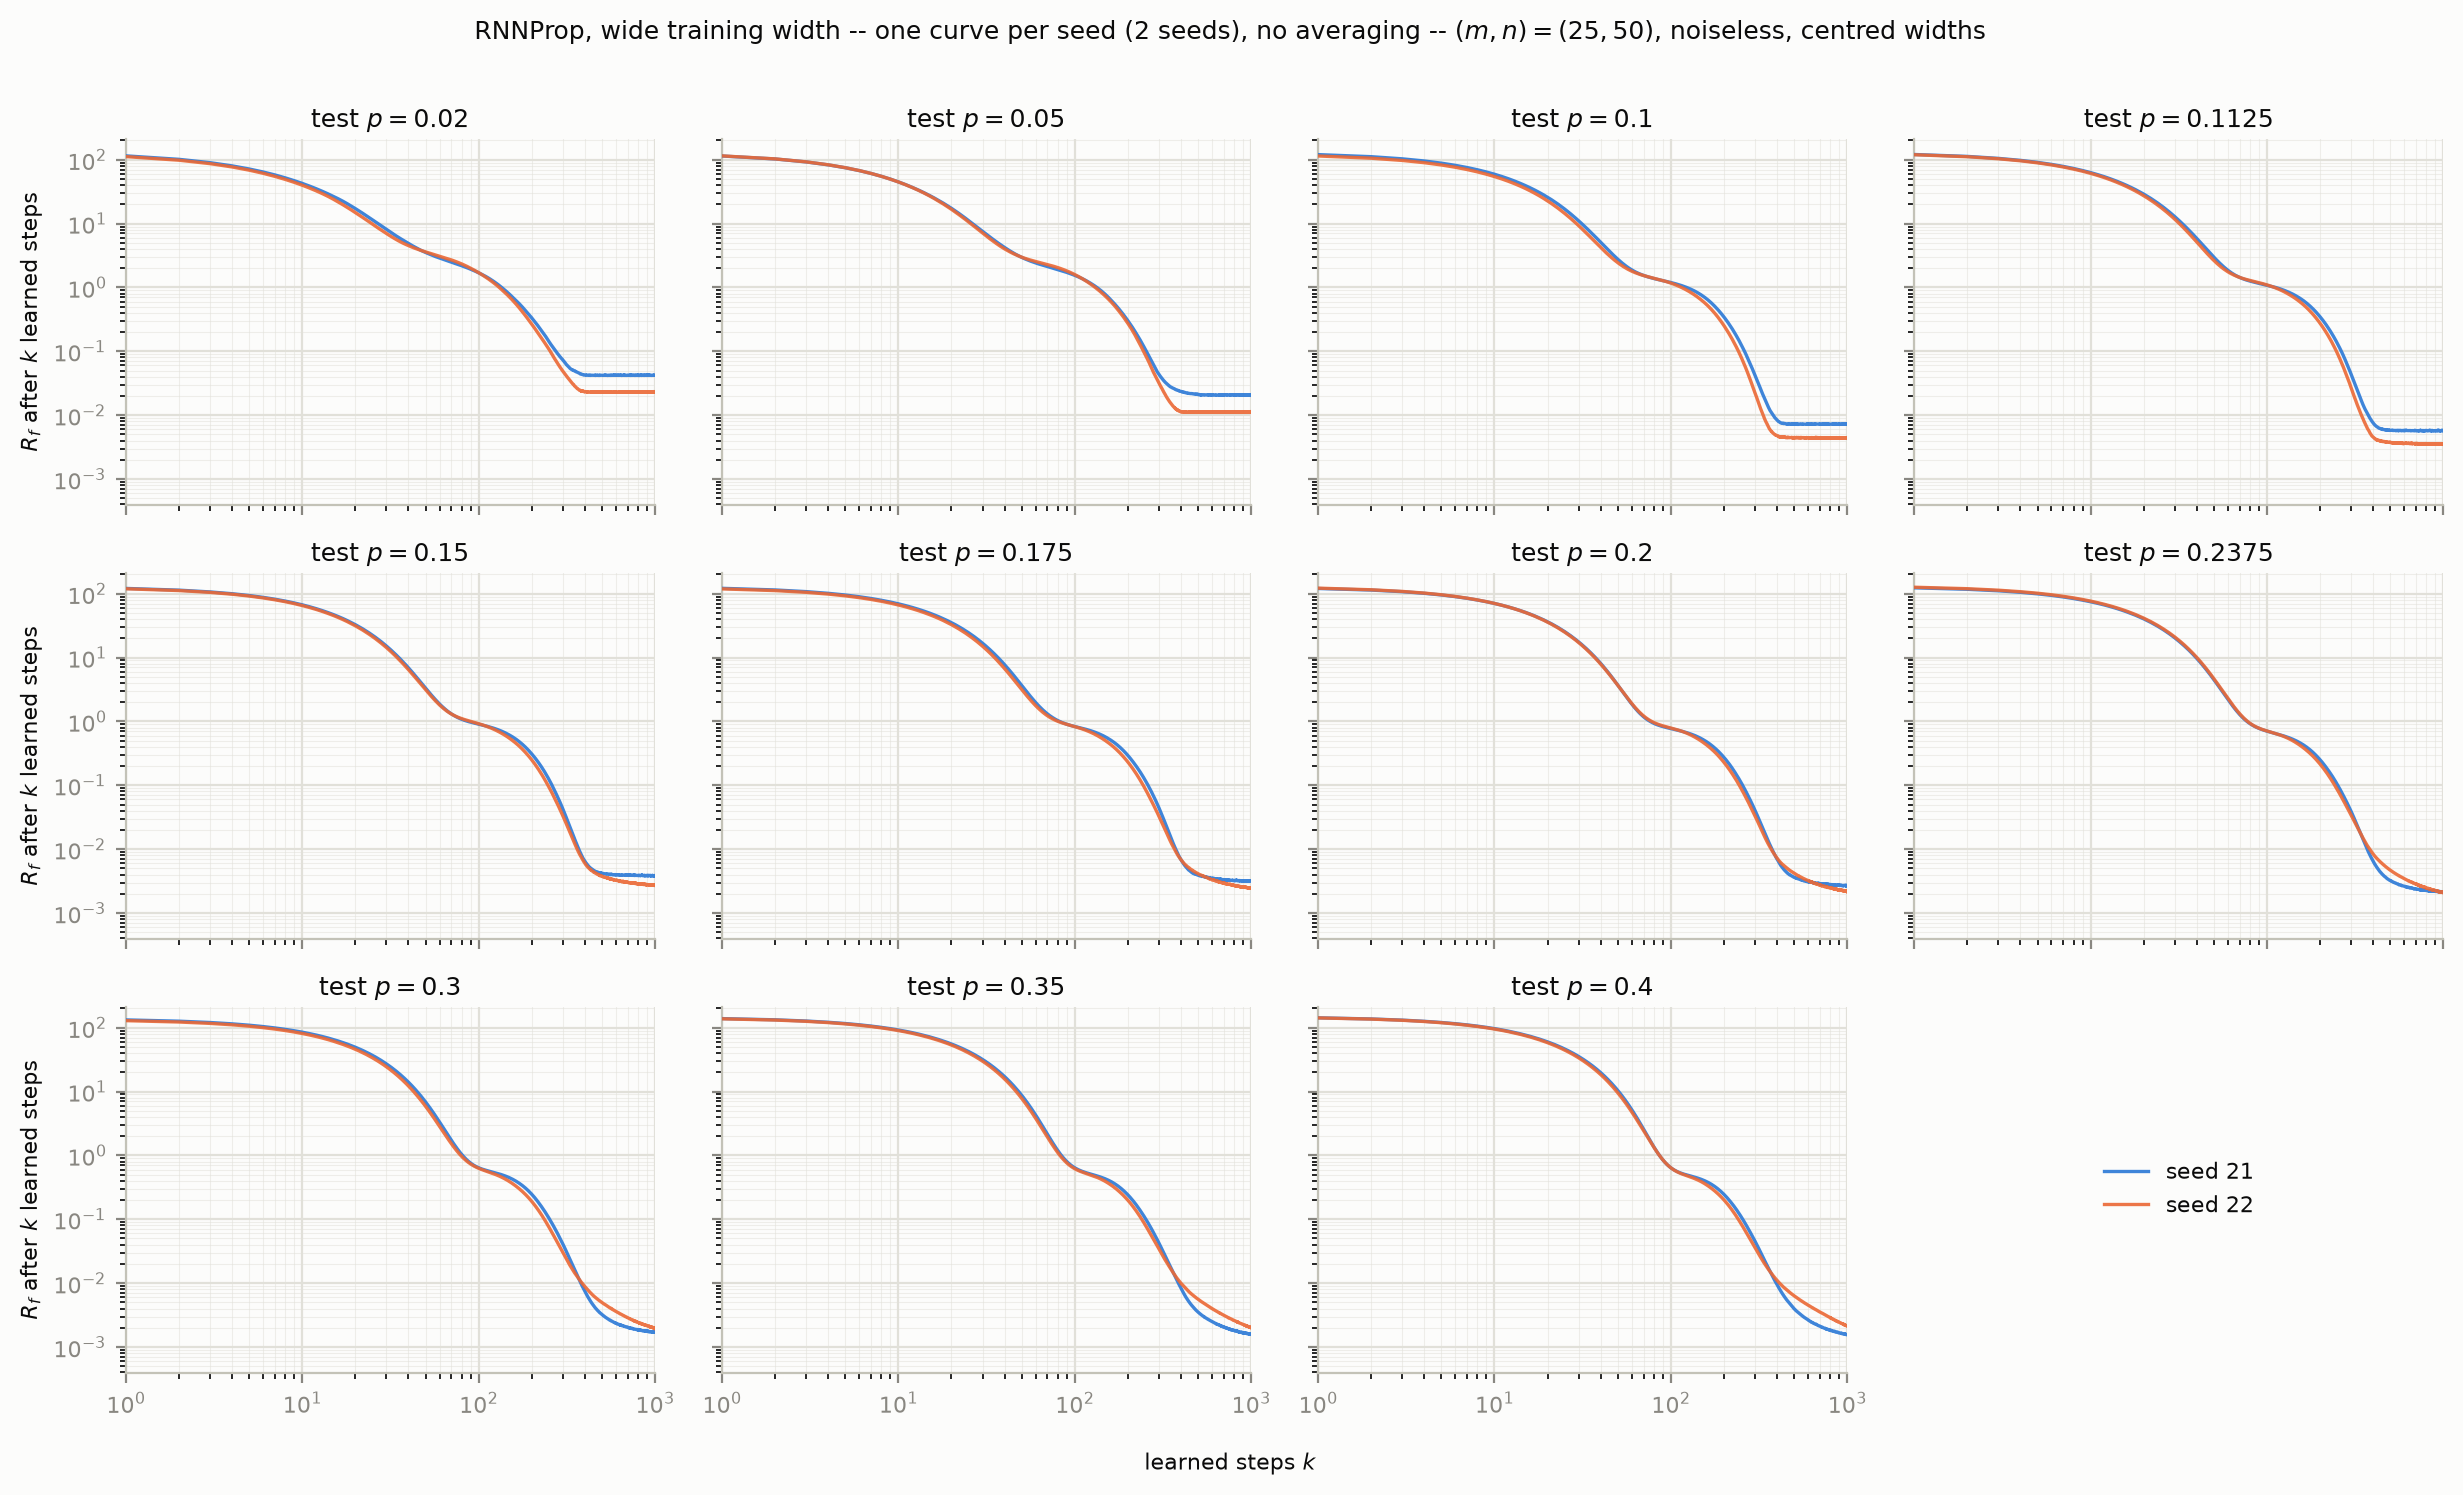
\includegraphics[width=\linewidth]{Figs/exp2_try2/rnnprop_seed_curves_exp2_try2_wide.png}
  \caption{Wide ($p \in [0.05, 0.30]$)}
  \label{fig:rnnprop-seed-curves-exp2-try2-wide}
\end{subfigure}\\[6pt]
\caption{L2O-RNNProp, modified relative loss $R_f$ (Eq.~10) against learned steps, $(m,n) = (25, 50)$, noiseless, centred widths. One curve per training seed (2 independently trained optimizers per width), no averaging; one panel per test sparsity $p$. The curves of different seeds agree closely for the first $\sim$100--200 steps and separate only on the plateau: the early trajectory is set by the architecture's normalised inputs and bounded ($\tanh \times 0.01$) output rather than by the learned weights.}
\label{fig:rnnprop-seed-curves-exp2-try2}
\end{figure}

\begin{figure}[htbp]
\centering
\begin{subfigure}[t]{\linewidth}
  \centering
  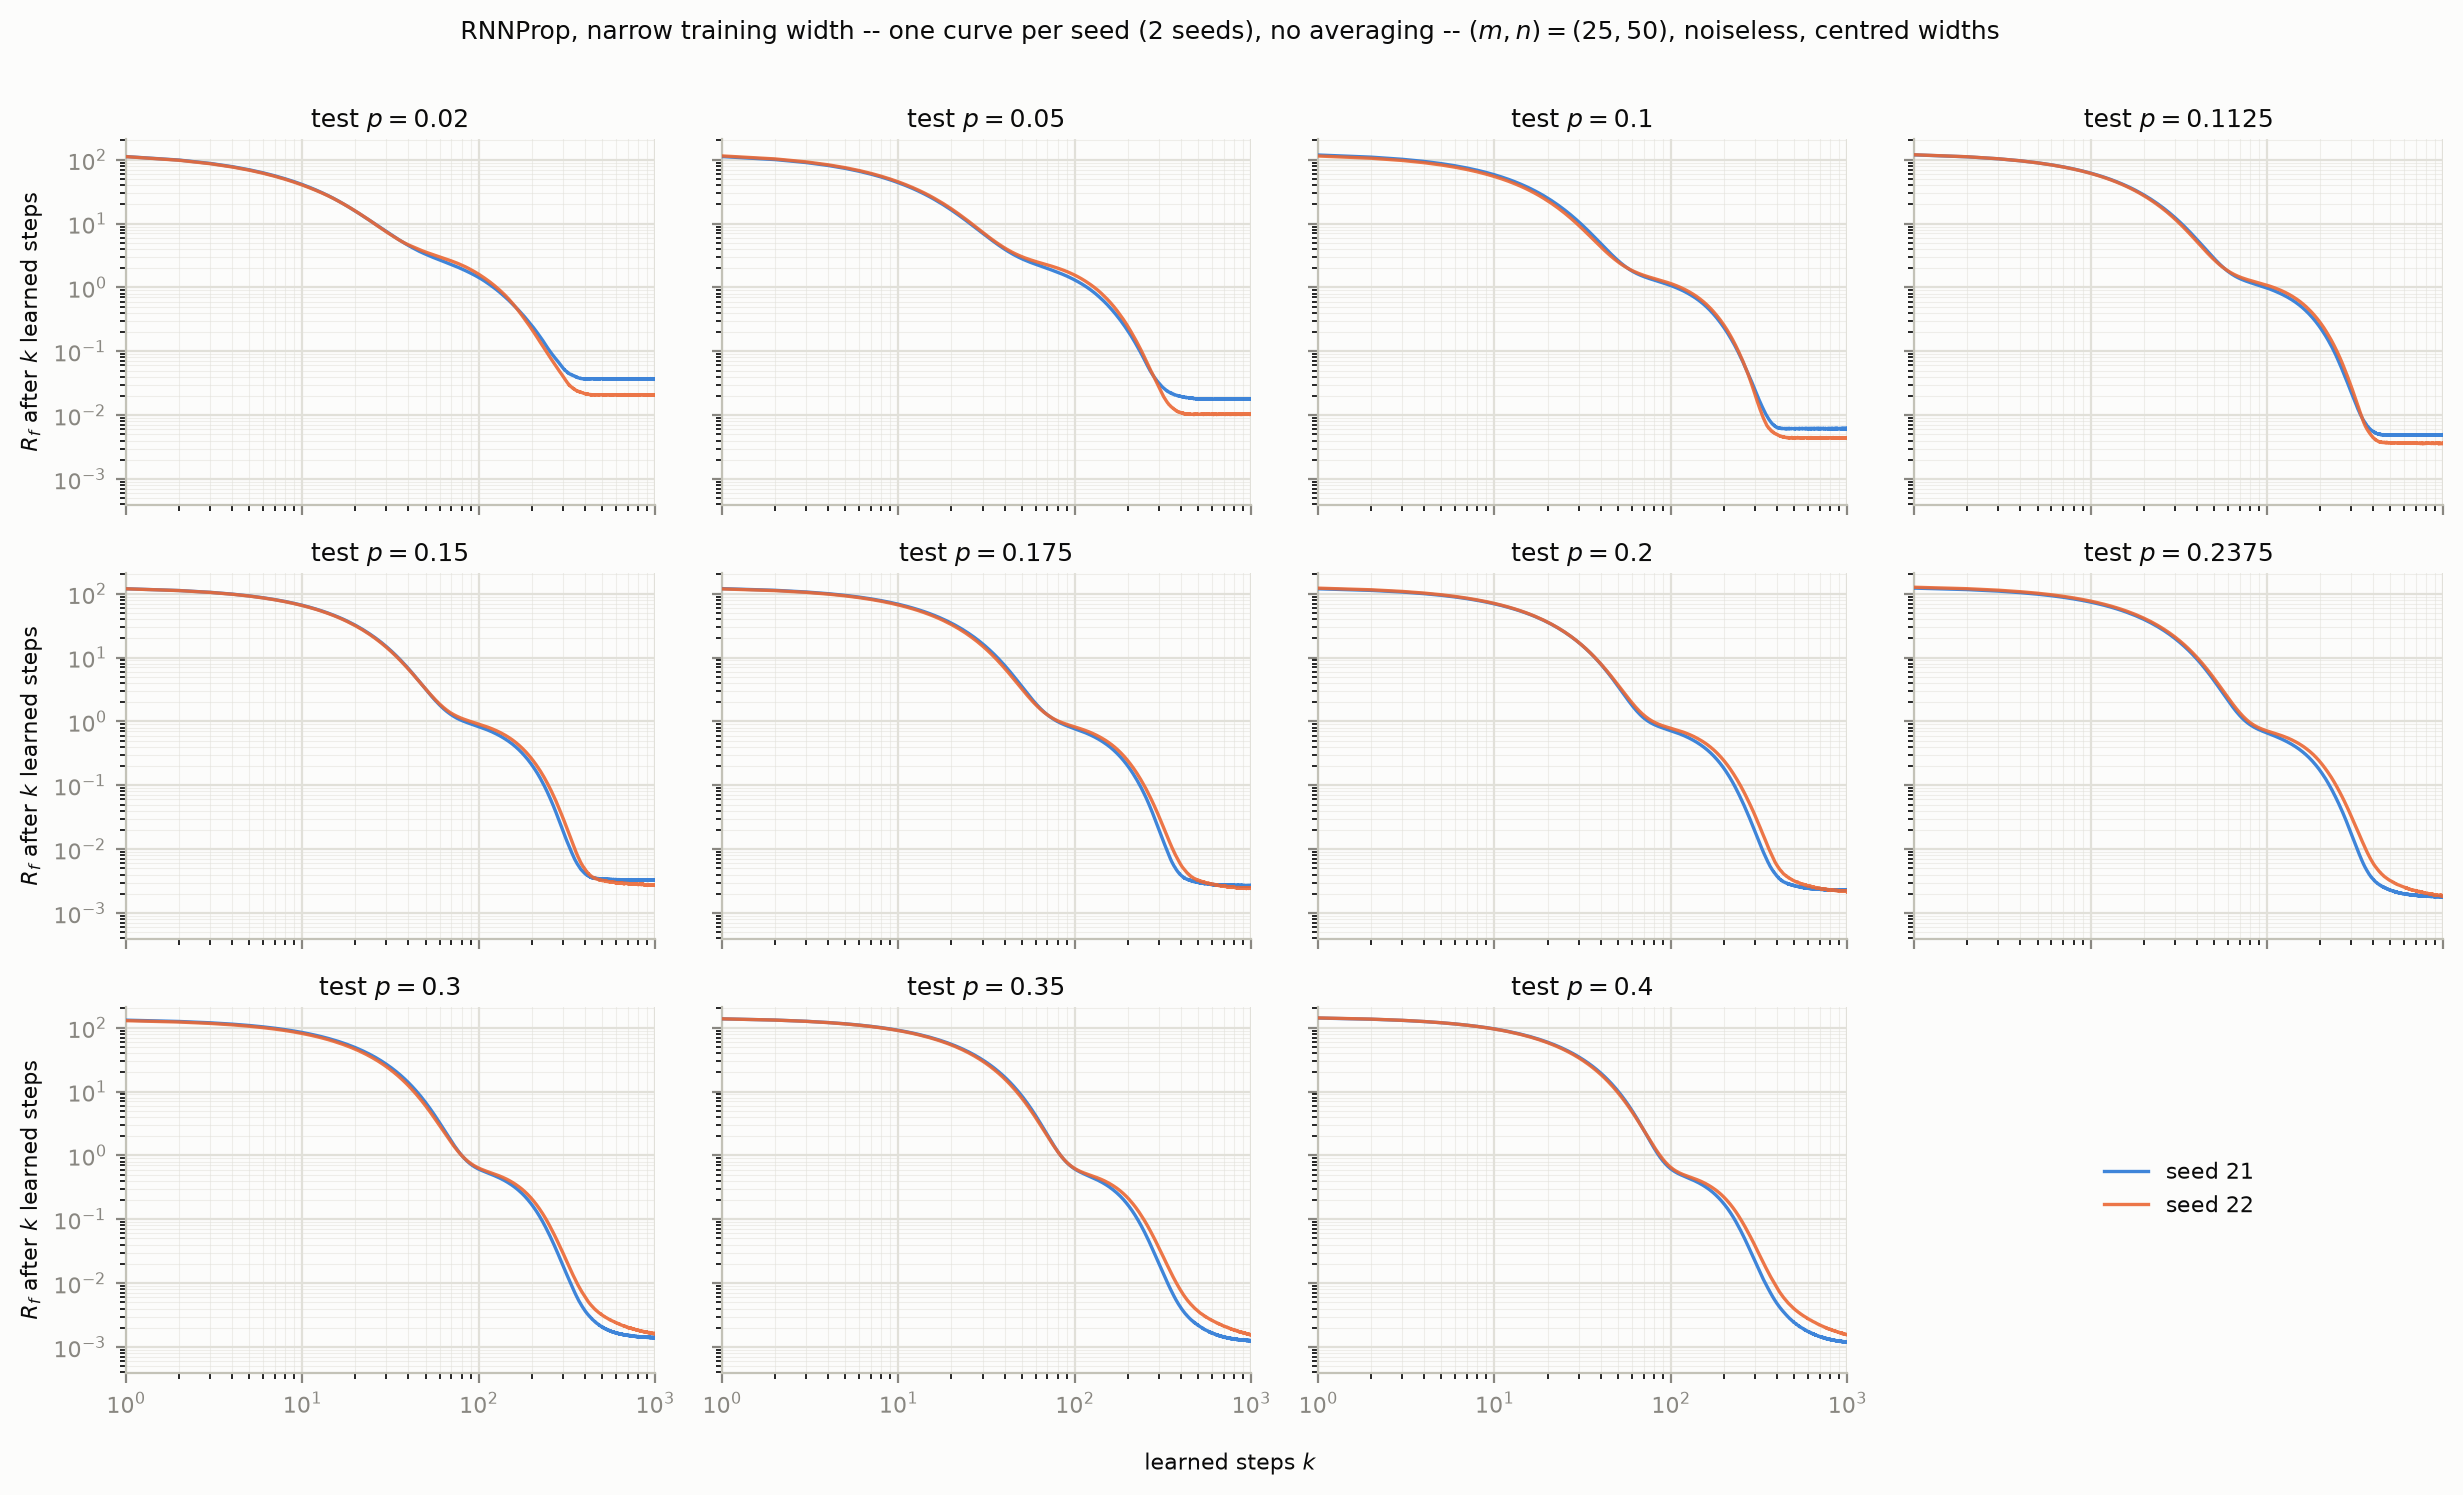
\includegraphics[width=\linewidth]{Figs/exp2_try2/rnnprop_seed_curves_exp2_try2_narrow.png}
  \caption{Narrow ($p = 0.175$)}
  \label{fig:rnnprop-seed-curves-exp2-try2-narrow}
\end{subfigure}\\[6pt]
\begin{subfigure}[t]{\linewidth}
  \centering
  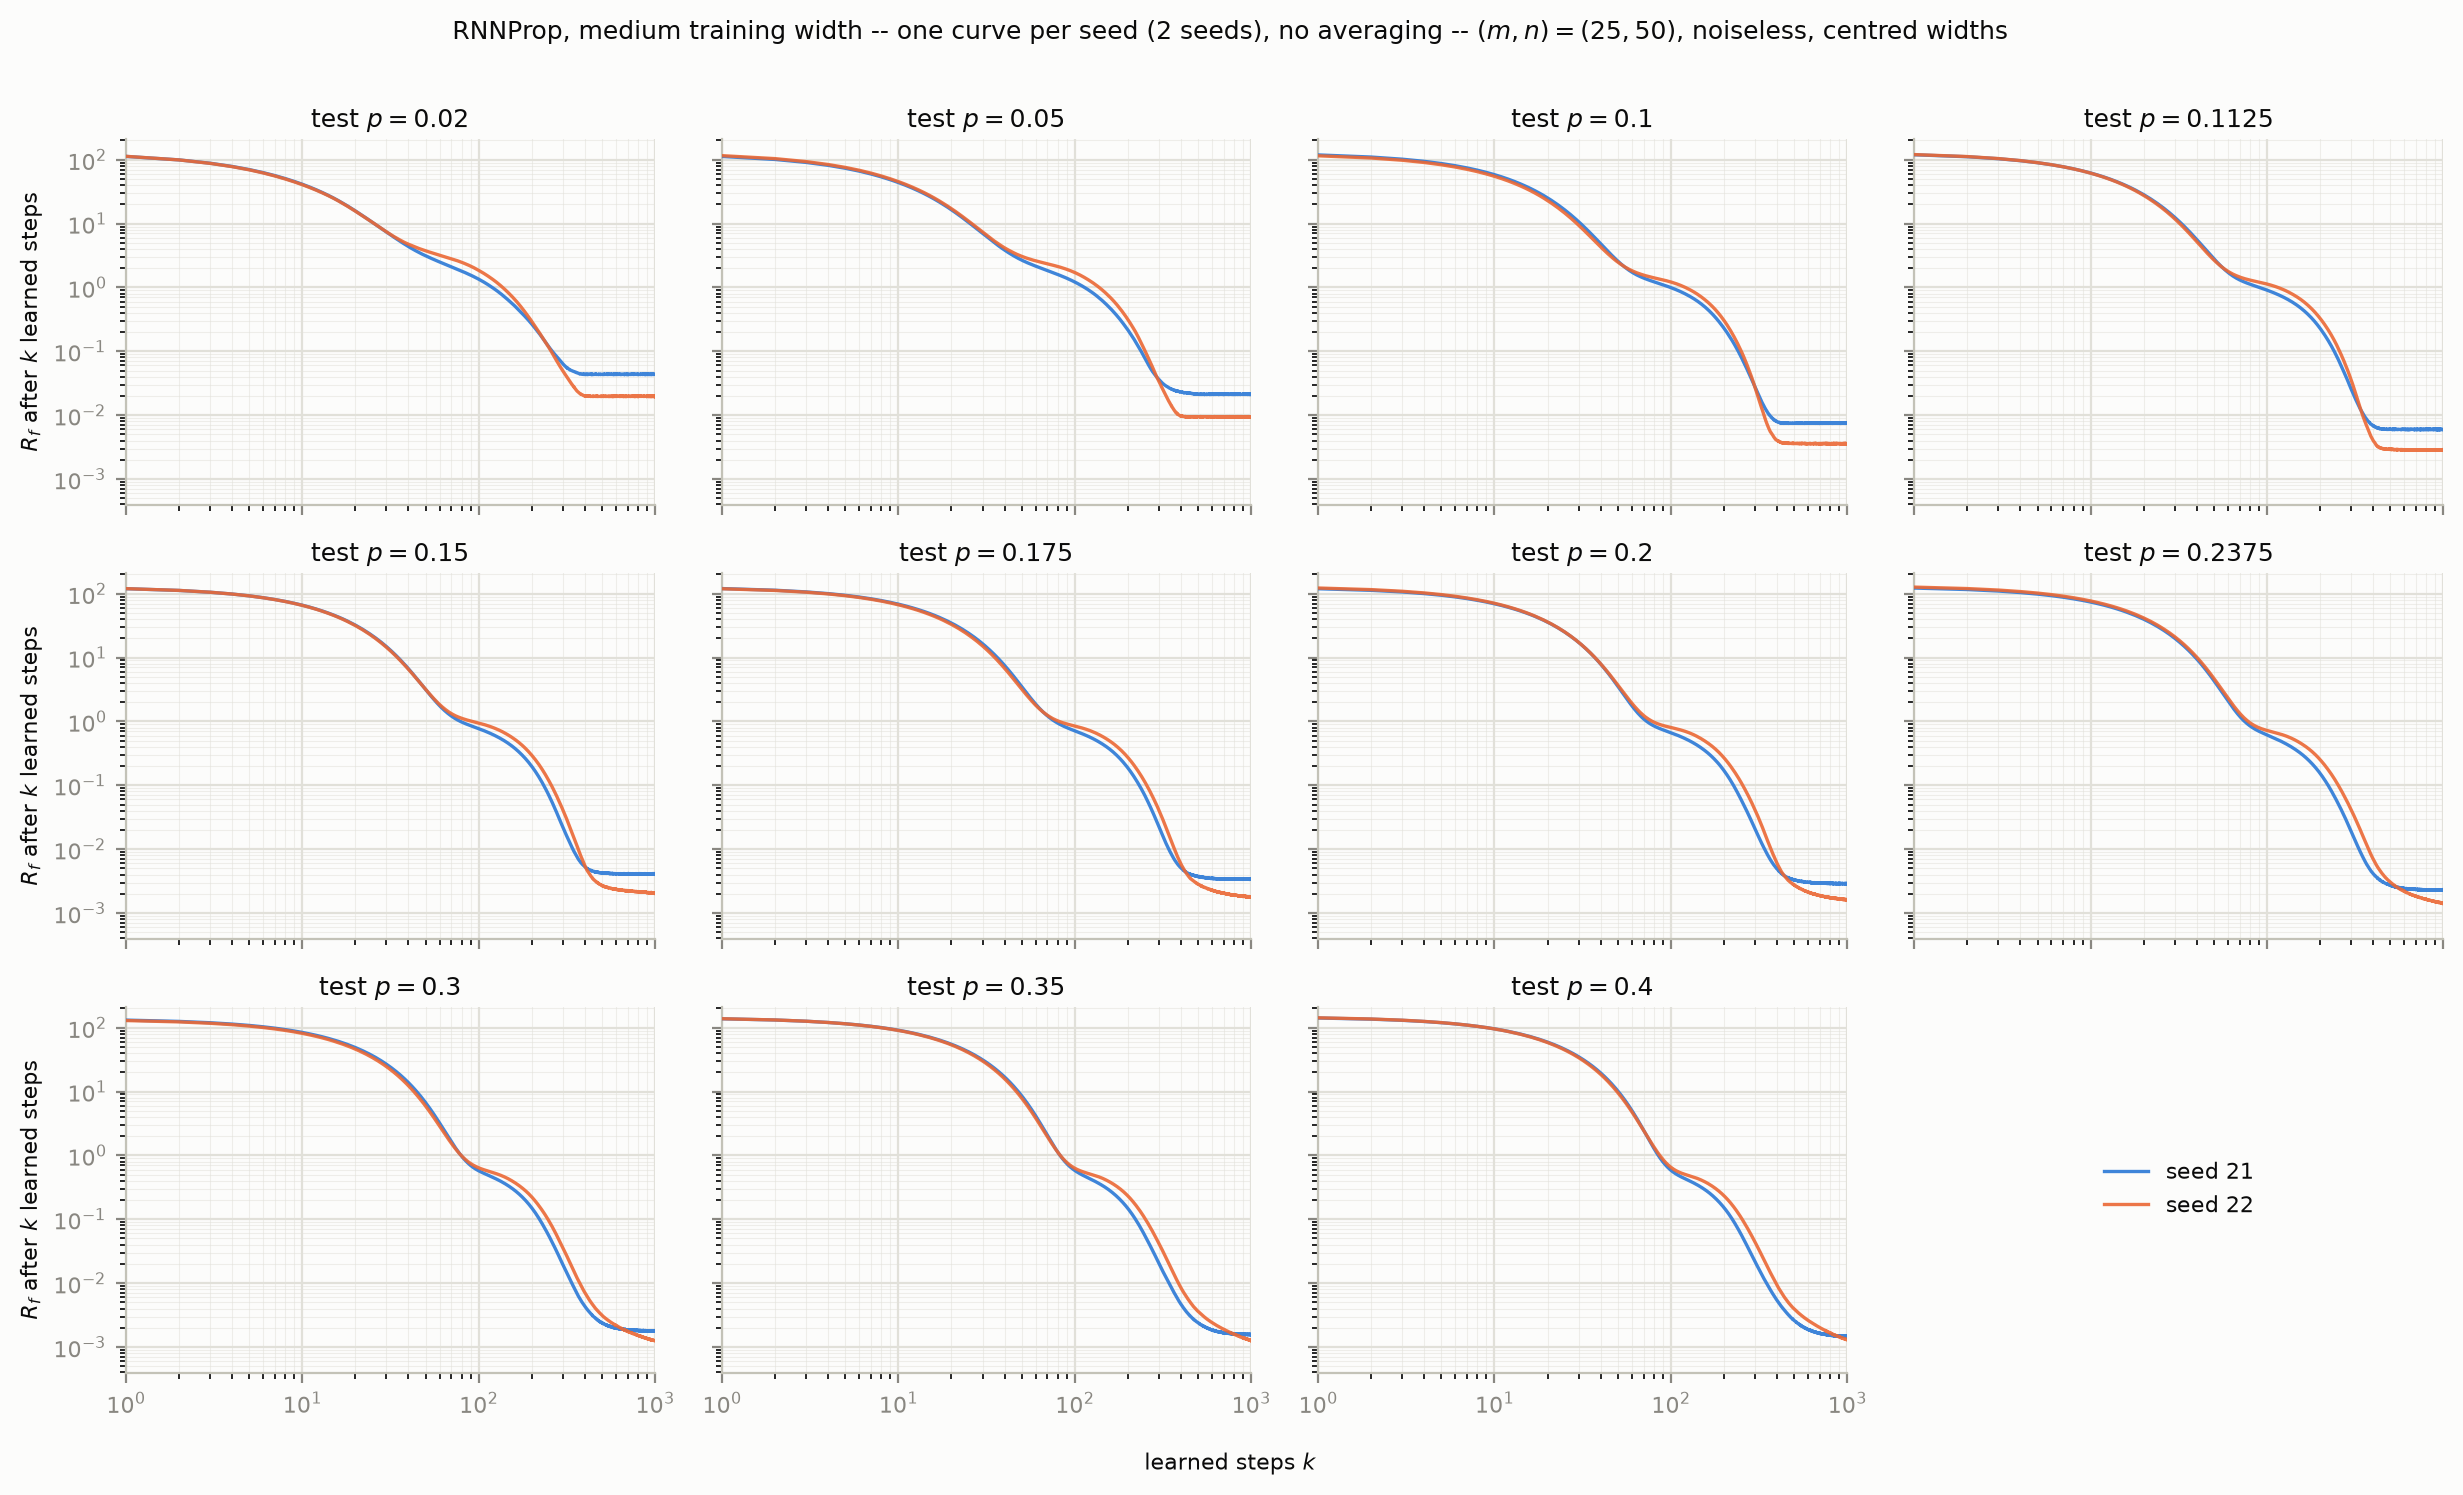
\includegraphics[width=\linewidth]{Figs/exp2_try2/rnnprop_seed_curves_exp2_try2_medium.png}
  \caption{Medium ($p \in [0.1125, 0.2375]$)}
  \label{fig:rnnprop-seed-curves-exp2-try2-medium}
\end{subfigure}\\[6pt]
\begin{subfigure}[t]{\linewidth}
  \centering
  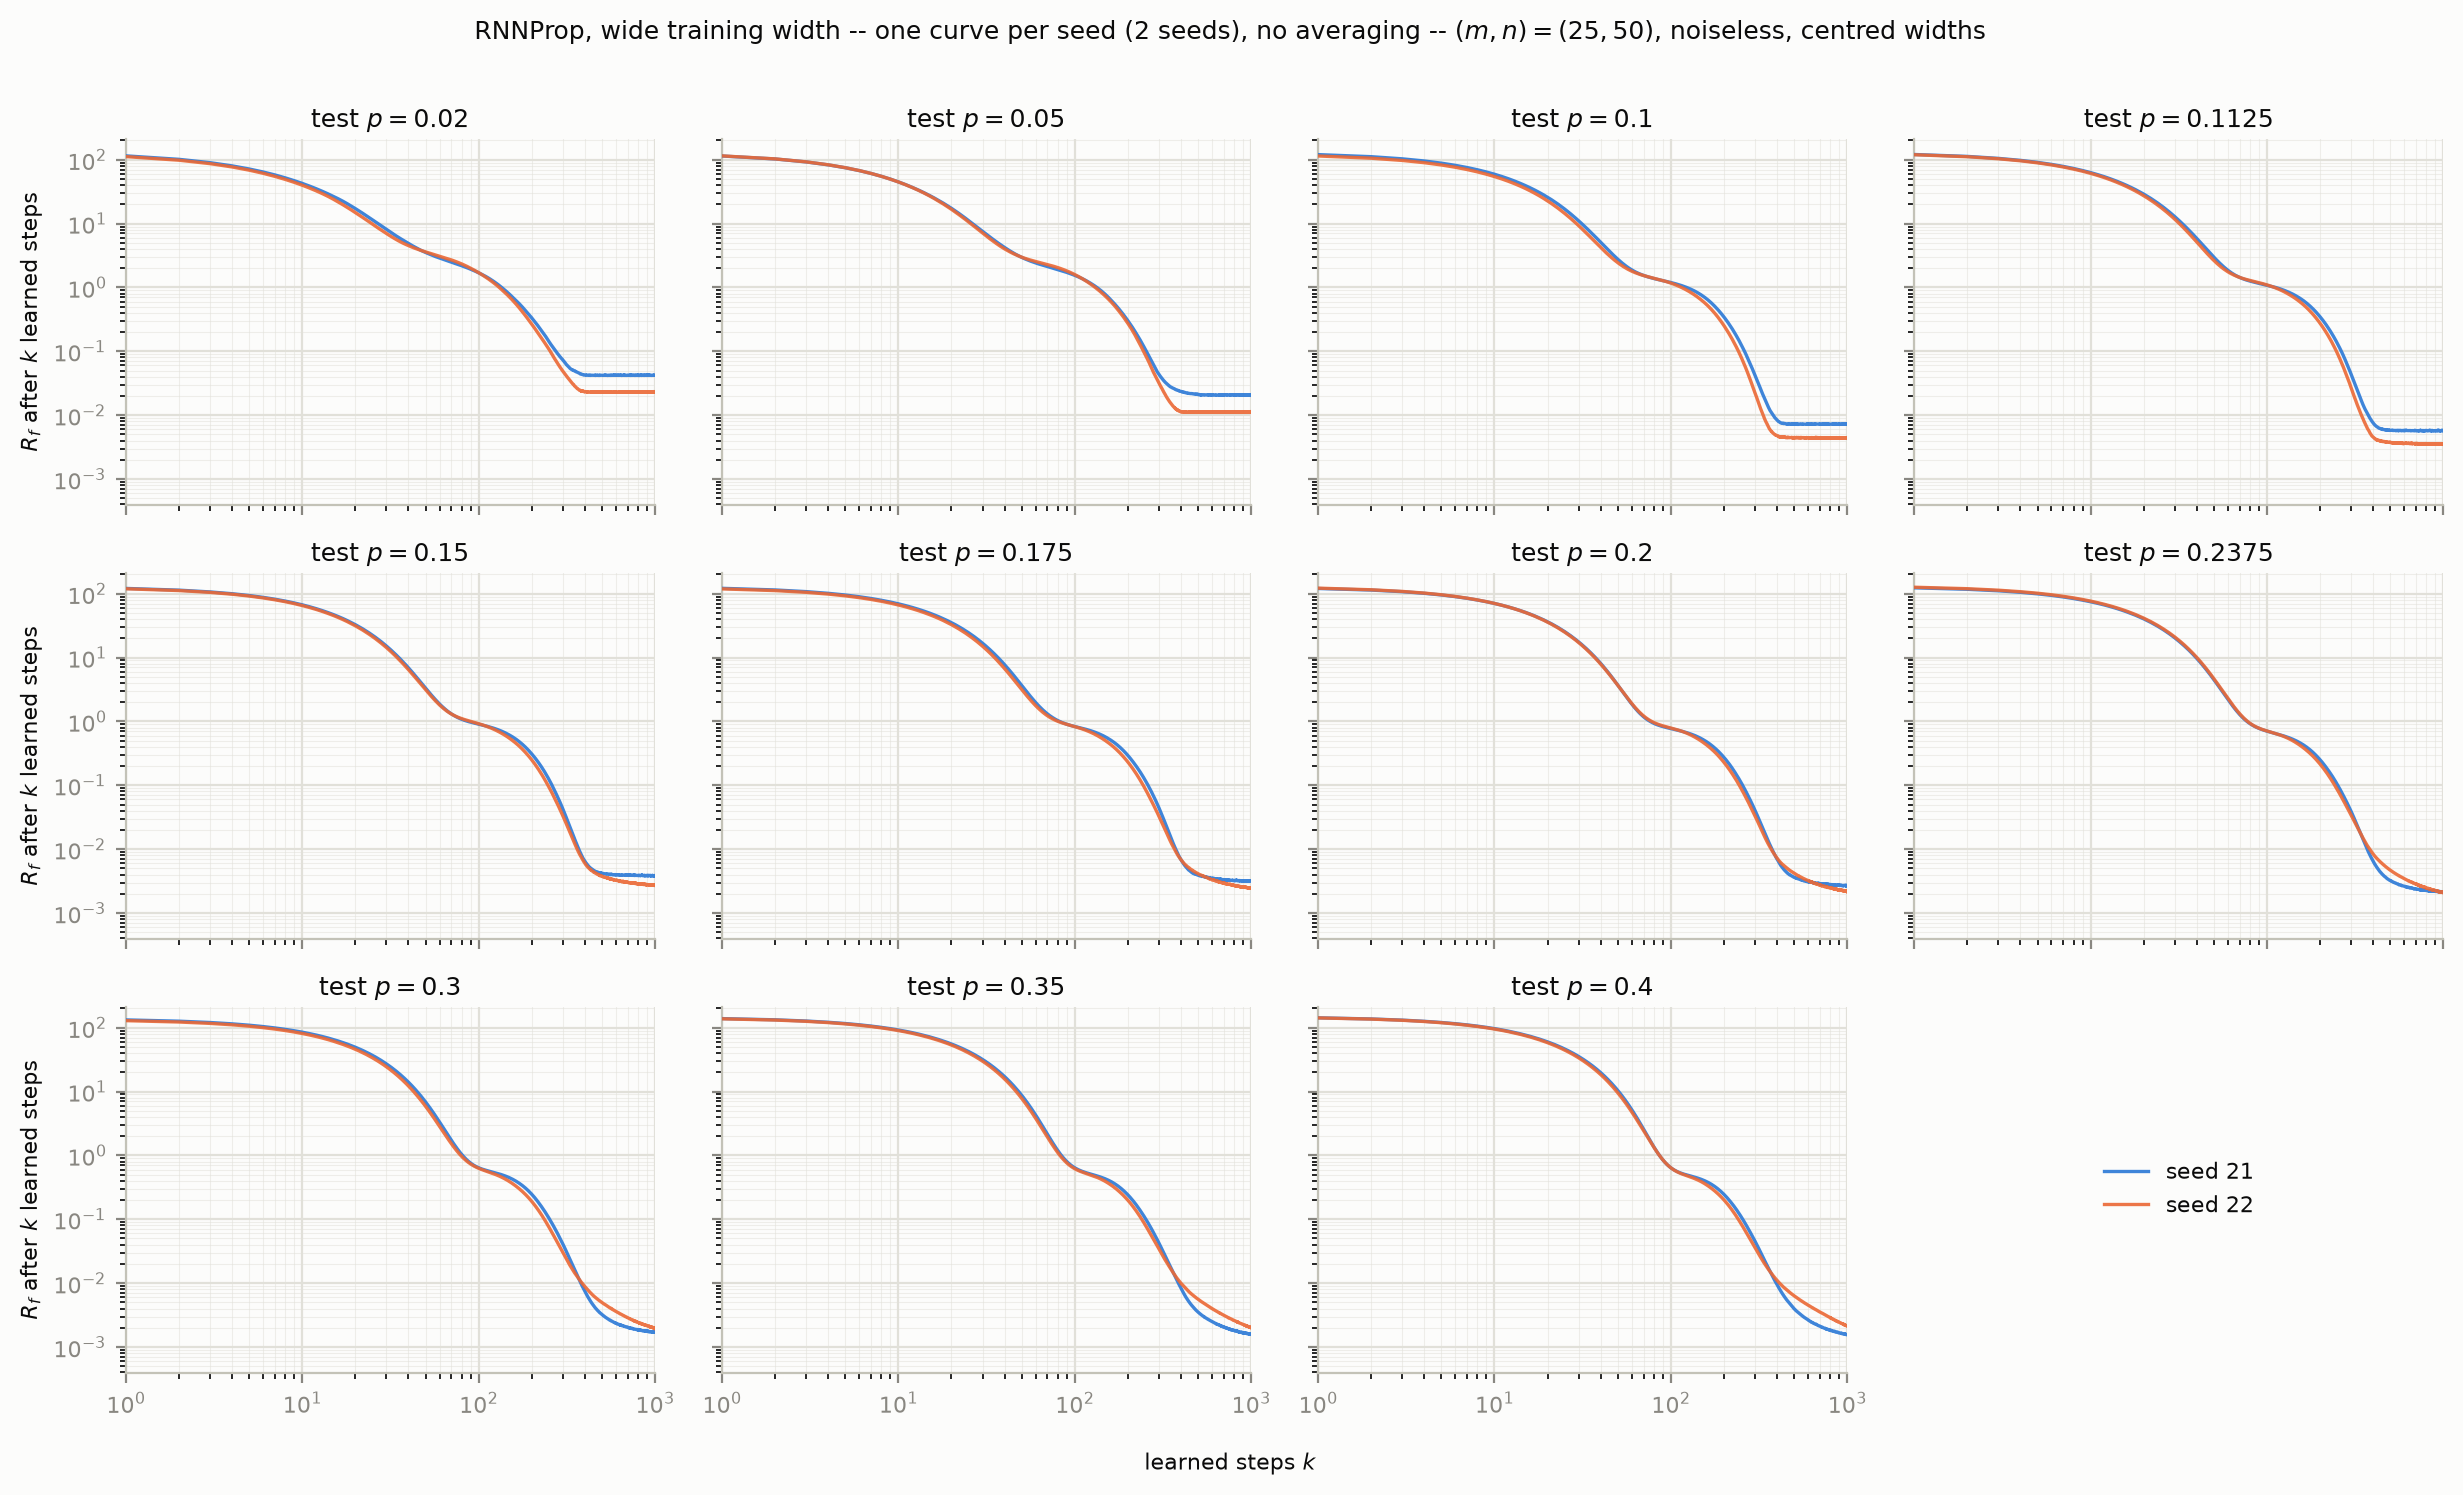
\includegraphics[width=\linewidth]{Figs/exp2_try2/rnnprop_seed_curves_exp2_try2_wide.png}
  \caption{Wide ($p \in [0.05, 0.30]$)}
  \label{fig:rnnprop-seed-curves-exp2-try2-wide}
\end{subfigure}\\[6pt]
\caption{L2O-RNNProp, modified relative loss $R_f$ (Eq.~10) against learned steps, $(m,n) = (25, 50)$, noiseless, centred widths. One curve per training seed (2 independently trained optimizers per width), no averaging; one panel per test sparsity $p$. The curves of different seeds agree closely for the first $\sim$100--200 steps and separate only on the plateau: the early trajectory is set by the architecture's normalised inputs and bounded ($\tanh \times 0.01$) output rather than by the learned weights.}
\label{fig:rnnprop-seed-curves-exp2-try2}
\end{figure}
